%\setcounter{chapter}{50}
\chapter{Vision and Language}\label{chapter:VLMs}

\section{Introduction}

The last few decades have seen enormous improvements in both computer vision and natural language processing. Naturally, there has been great interest in putting these two branches of artificial intelligence (AI) together.

At first it might seem like vision has little to do with language. This is what you might conclude if you see the role of language as just being about communication. However, another view on language is that it is a representation of the world around us, and this representation is one the brain uses extensively for higher-level cognition~\cite{fodor1975language}. Visual perception is also about representing the world around us and forming mental models that act as a substrate for reasoning and decision making. From this perspective, both language and vision are trying to solve more or less the same problem.

It turns out this view is quite powerful, and indeed language and vision can help each other in innumerable ways. This chapter is about some of the ways language can improve vision systems, and also how vision systems can support language systems.

\section{Background: Representing Text as Tokens}
In order to understand \index{Vision-language models}\textbf{vision-language models} (\textbf{VLMs}) we first need to understand a bit about \index{Language models}\textbf{language models}. There are many ways to model language and indeed there is a whole field that studies this, called \index{Natural language processing}\textbf{natural language processing} (\textbf{NLP}). We will present just one way, which follows almost exactly the same format as modern computer vision systems: tokenize the text, then process it with a transformer. In \chap{\ref{chapter:transformers}} we saw how to apply transformers to images and now we will see how to apply them to text.
\marginnote{Language models analyze or synthesize languages, including human languages like English or Chinese, programming languages like Python and C++, and scripting languages like Latex or HTML. Some communities reserve the term for models of \textit{human} languages, but we will use the term in a broader sense and include other kinds of languages too.}[-2.4cm]

The amazing thing about transformers is that they work well for a wide variety of data types: in fact, the same architectures that we saw in \chap{\ref{chapter:transformers}} also works for text processing. To apply transformers to a new data modality may require nothing more than
figuring out how to represent that data as numbers.

So our first question is, how can we represent text as numbers? One option, which we have already seen, is to use a word-level encoding scheme, mapping each word in our vocabulary to a unique one-hot code. This requires $K$-dimensional one-hot codes for a vocabulary of $K$ different words.

A disadvantage of this approach is that $K$ has to be very large to cover a language like English, which has a large vocabulary of over 100,000 possible words. This becomes even worse for computer languages, like Python. Programmers routinely name variables using made up words, which might never have been used before. We can't define a vocabulary large enough to cover all the strange strings programmers might come up with.

Instead, we could use a different strategy, where we assign a one-hot code to each \textit{character} in our vocabulary, rather than to each unique word. If we represent all alphanumeric characters and common punctuation marks in this way, this might only require a few dozen codes. The disadvantage here is that representing a single word now requires a sequence of one-hots rather than a single one-hot code, and we will have to model that sequence.

A happy middle ground can be achieved using \index{Byte-pair encoding}\textbf{byte-pair} encodings~\cite{gage1994new}. In this approach, we assign a one-hot code to each small chunk of text. The chunks are common substrings found in text, like ``th'' or ``ing.'' This strategy is popular in language models like the \index{Generative pretrained transformer}\textbf{generative pretrained transformer} (\textbf{GPT}) series~\cite{brown2020language} and the \index{Contrastive language-image pretraining}\textbf{contrastive language-image pretraining} (\textbf{CLIP}) model~\cite{radford2021learning} that we will learn about in \sect{\ref{sec:VLMs:CLIP}}.

Once we have converted text into a sequence of one-hot codes, the next step is to convert these into tokens via a projection, $\mathbf{W}_{\texttt{tokenize}}$, from the one-hot dimensionality ($K$) to a target dimensionality for token code vectors ($d$). \Fig{\ref{fig:VLMs:tokenizing_text}} shows these steps for converting an input string to tokens. For simplicity, we show word-level one-hot encoding rather than byte-pair encoding.
\begin{figure}[h]
    \centerline{
        \begin{tikzpicture}
            %
            %% Image encoder
            \def\Nnodes{3}
            \def\layerheight{1.2}
            \def\neuronrad{0.3}
            \def\neuronstep{0.7}
            % text inputs
            \node [rotate=45] at (\neuronstep,-\layerheight) {\small \texttt{A}};
            \node [rotate=45] at (\neuronstep*2,-\layerheight) {\small \texttt{yellow}};
            \node [rotate=45] at (\neuronstep*3,-\layerheight) {\small \texttt{bird}};
            \node at (\neuronstep*4,-\layerheight) {\small \ldots};
            % projection notation
            \node at (\neuronstep*4.5-\neuronrad/4,2*\layerheight/3) {$\mathbf{W}_{\texttt{tokenize}}$};
            % one-hots
            \foreach \x in {1,...,\Nnodes} {
                    \draw (\neuronstep*\x-\neuronrad/4,\layerheight-\layerheight-\neuronrad) rectangle ++(\neuronrad/2,\neuronrad*3);
                }
            \draw[decorate,decoration={brace, amplitude=5pt, angle=0}] (\neuronstep-\neuronrad/2,-\neuronrad) -- (\neuronstep-\neuronrad/2,-\neuronrad+\neuronrad*3);
            \node[left] at (\neuronstep-\neuronrad*2.5,\neuronstep/2) {one-hots};
            \node[left] at (\neuronstep-\neuronrad,\neuronstep/2-\neuronrad*1.5) {($K$-dimensional)};
            % tokens
            \foreach \x in {1,...,\Nnodes} {
                    \draw (\neuronstep*\x-\neuronrad/4,\layerheight*2-\layerheight) rectangle ++(\neuronrad/2,\neuronrad*2);
                }
            \draw[decorate,decoration={brace, amplitude=5pt, angle=0}] (\neuronstep-\neuronrad/2,\layerheight) -- (\neuronstep-\neuronrad/2,-\neuronrad+\neuronrad*3+\layerheight);
            \node[left] at (\neuronstep-\neuronrad*2.5,\neuronstep/2+\layerheight) {tokens};
            \node[left] at (\neuronstep-\neuronrad,\neuronstep/2-\neuronrad*1.5+\layerheight) {($d$-dimensional)};
            % text to one-hots arrow
            \foreach \x in {1,...,\Nnodes} {
                    \draw [thick] [nn_edge] (\neuronstep*\x,\neuronrad-\layerheight) -- (\neuronstep*\x,\layerheight-\neuronrad-\layerheight);
                }
            % one-hots to token vectors arrow
            \foreach \x in {1,...,\Nnodes} {
                    \draw [thick] [nn_edge] (\neuronstep*\x,\neuronrad*2) -- (\neuronstep*\x,\layerheight);
                }
        \end{tikzpicture}
    }
    \caption{Tokenizing text. Note that these steps can be implemented with a lookup table that simply stores the token code vector for each unique item in our vocabulary.}
    \label{fig:VLMs:tokenizing_text}
\end{figure}

%Now that we have represented text as a set of vectors (a sequence of one-hot codes), we can project each vector into a token and text becomes represented as a sequence of tokens. This is the format that transformers take as input and produce as output. 

These steps map text to tokens, which can be input into transformers. To handle the output side, where we produce text as an output, we need to convert tokens back to text. The most common way to do this is to use an autoregressive model that predicts each next item in our vocabulary (word/character/byte-pair) given the sequence generated so far. Each prediction step can be modeled as a softmax over all $K$ possible items in our vocabulary. We will see a specific architecture that does this in \sect{\ref{sec:VLMs:im2text}}.


\section{Learning Visual Representations from Language Supervision}\label{sec:VLMs:CLIP}
\index{Contrastive language-image pretraining}

In \chap{\ref{chapter:representation_learning}}, we saw that one approach of learning visual representations is to set up a pretext task that requires arriving at a good representation of the scene. In this section we will revisit this idea, using language association as a pretext task for representation learning.

In fact this is not a new idea: historically, one of the most popular pretext tasks has been image classification, where an image is associated with one of $K$ nouns. In a sense, this is already a way of supervising visual representations from language. Of course, human languages are much more than just a set of $K$ nouns. This raises the question, could we use richer linguistic structure to supervise vision?

The answer is yes! And it works really well. Researchers have tried using all kinds of language structures to supervise vision systems, including adjectives and verbs~\cite{StatesAndTransformations}, words indicating relationships between objects~\cite{visualgenome}, and question-answer pairs~\cite{antol2015vqa}. What seems to work best, once you reach a certain scale of data and compute, is to just use \textit{all} the structure in language, and the simplest way to do this is to train a vision system that associates images with free-form natural language.

This is the idea of the highly popular CLIP system~\cite{radford2021learning}.\footnote{The idea of visual learning by image captioning actually has a long history before CLIP. One important early paper on this topic is \cite{ordonez2011im2text}.} CLIP is a contrastive method (see \sect{\ref{sec:representation_learning:contrastive_learning}}) in which one data view is the image and the other is a caption describing the image. Specifically, CLIP is a form of contrastive learning from co-occurring visual and linguistic views that is formulated as follows:
\begin{center}
    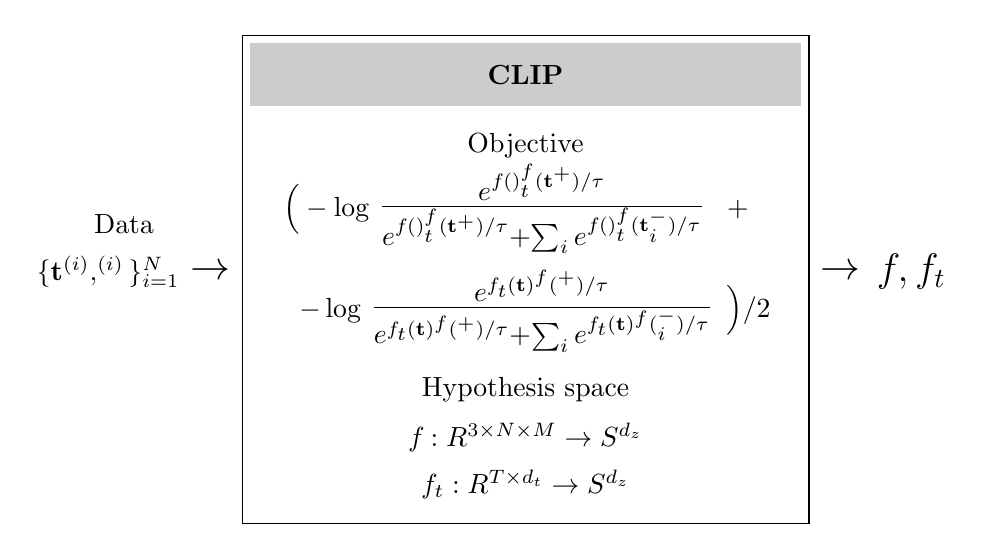
\begin{tikzpicture}
        \draw (0,-1.0) rectangle (7.2,5.2); % outer box
        \fill[black!20] (0.1,4.3) rectangle (7.1,5.1); % gray box
        \node[] at (3.6,4.7) {{\bf CLIP}};
        \node[] at (3.6,3.8) {Objective}; \node[] at (3.48,3.0) {$\Big(-\log$ {\Large $\frac{e^{f_{\img}(\boldimg)^\transpose f_{t}(\mathbf{t}^+)/\tau}}{e^{f_{\img}(\boldimg)^\transpose f_t(\mathbf{t}^+)/\tau} + \sum_i e^{f_{\img}(\boldimg)^\transpose f_t(\mathbf{t}_i^-)/\tau}}$ } $+ $};%{$(\texttt{InfoNCE}(\boldimg, \mathbf{t}^+, \{\mathbf{t}_i^-\}_{i=1}^N) +$}; 
        \node[] at (3.72,1.7) {$-\log$ {\Large $\frac{e^{f_t(\mathbf{t})^\transpose f_{\img}(\boldimg^+)/\tau}}{e^{f_{t}(\mathbf{t})^\transpose f_{\img}(\boldimg^+)/\tau} + \sum_i e^{f_t(\mathbf{t})^\transpose f_{\img}(\boldimg_i^-)/\tau}}$ }$\Big)/2$};%{$\texttt{InfoNCE}(\mathbf{t}, \boldimg^+, \{\boldimg_i^-\}_{i=1}^N))/2$};
            \node[] at (3.6,0.7) {Hypothesis space}; \node[] at (3.6,0.1) {$f_{\img}: \mathbb{R}^{3 \times N \times M} \rightarrow \mathbb{S}^{d_z}$}; \node[] at (3.6,-0.5) {$f_t: \mathbb{R}^{T \times d_t} \rightarrow \mathbb{S}^{d_z}$};
            \node[] at (-1.5,2.8) {Data};
            \node[] at (-1.7,2.2) {$\{\mathbf{t}^{(i)}, \boldimg^{(i)}\}_{i=1}^N$};
        \node[] at (-0.4,2.2) {{\Large  $ \rightarrow$}};
        \node[] at (8.5,2.2) {{\Large $f_{\img}, f_t$}};
        \node[] at (7.6,2.2) {{\Large  $ \rightarrow$}};
        %
        \useasboundingbox (-2,-0.1) rectangle (9,5.3);
    \end{tikzpicture}
\end{center}
where $\boldimg$ represents an image, $\mathbf{t}$ represents text, $\mathbb{S}^{d_z}$ represents the space of unit vectors of dimensionality $d_z$ (i.e., the surface of the $[d_z-1]$-dimensional hypersphere), $f_{\img}$ is the image encoder, $f_t$ is the text encoder, image inputs are represented as $[3 \times N \times M]$ pixel arrays, text inputs are represented as $d_t$ dimensional tokens, and $d_z$ is the embedding dimensionality. Notice that the objective is a symmetric version of the InfoNCE loss defined in \eqn{\ref{eqn:representation_learning:infonce}}. Also notice that $f_\img$ and $f_t$ both output unit vectors (which is achieved using $L_2$-normalization before computing the objective); this ensures that the denominator cannot dominate by pushing negative pairs infinitely far apart.

\Fig{\ref{fig:vision_and_language:clip_training}} visually depicts how CLIP is trained. First we sample a batch of $N$ language-image pairs, $\{\mathbf{t}^{(i)}, \boldimg^{(i)}\}_{i=1}^N$ ($N=6$ in the figure). Next we embed measure the dot product between all these text strings and images using a language encoder $f_t$ and an image encoder $f_\img$, respectively. This produces a set of text embeddings $\{\mathbf{z}^{(i)}_t\}_{i=1}^N$ and a set of image embeddings $\{\mathbf{z}^{(i)}_\img\}_{i=1}^N$. To compute the loss, we take the dot product $\mathbf{z}^{(i)}_\img \cdot \mathbf{z}^{(j)}_t$ for all $i, j \in \{1,\ldots,6\}$. Terms for which $i \neq j$ are the negative pairs and we seek to minimize these dot products (denominator of the loss); terms for which $i == j$ are the positive pairs and we seek to maximize these dot product (they appear in both the numerator and denominator of the loss).
\begin{figure}[h]
    \centerline{
        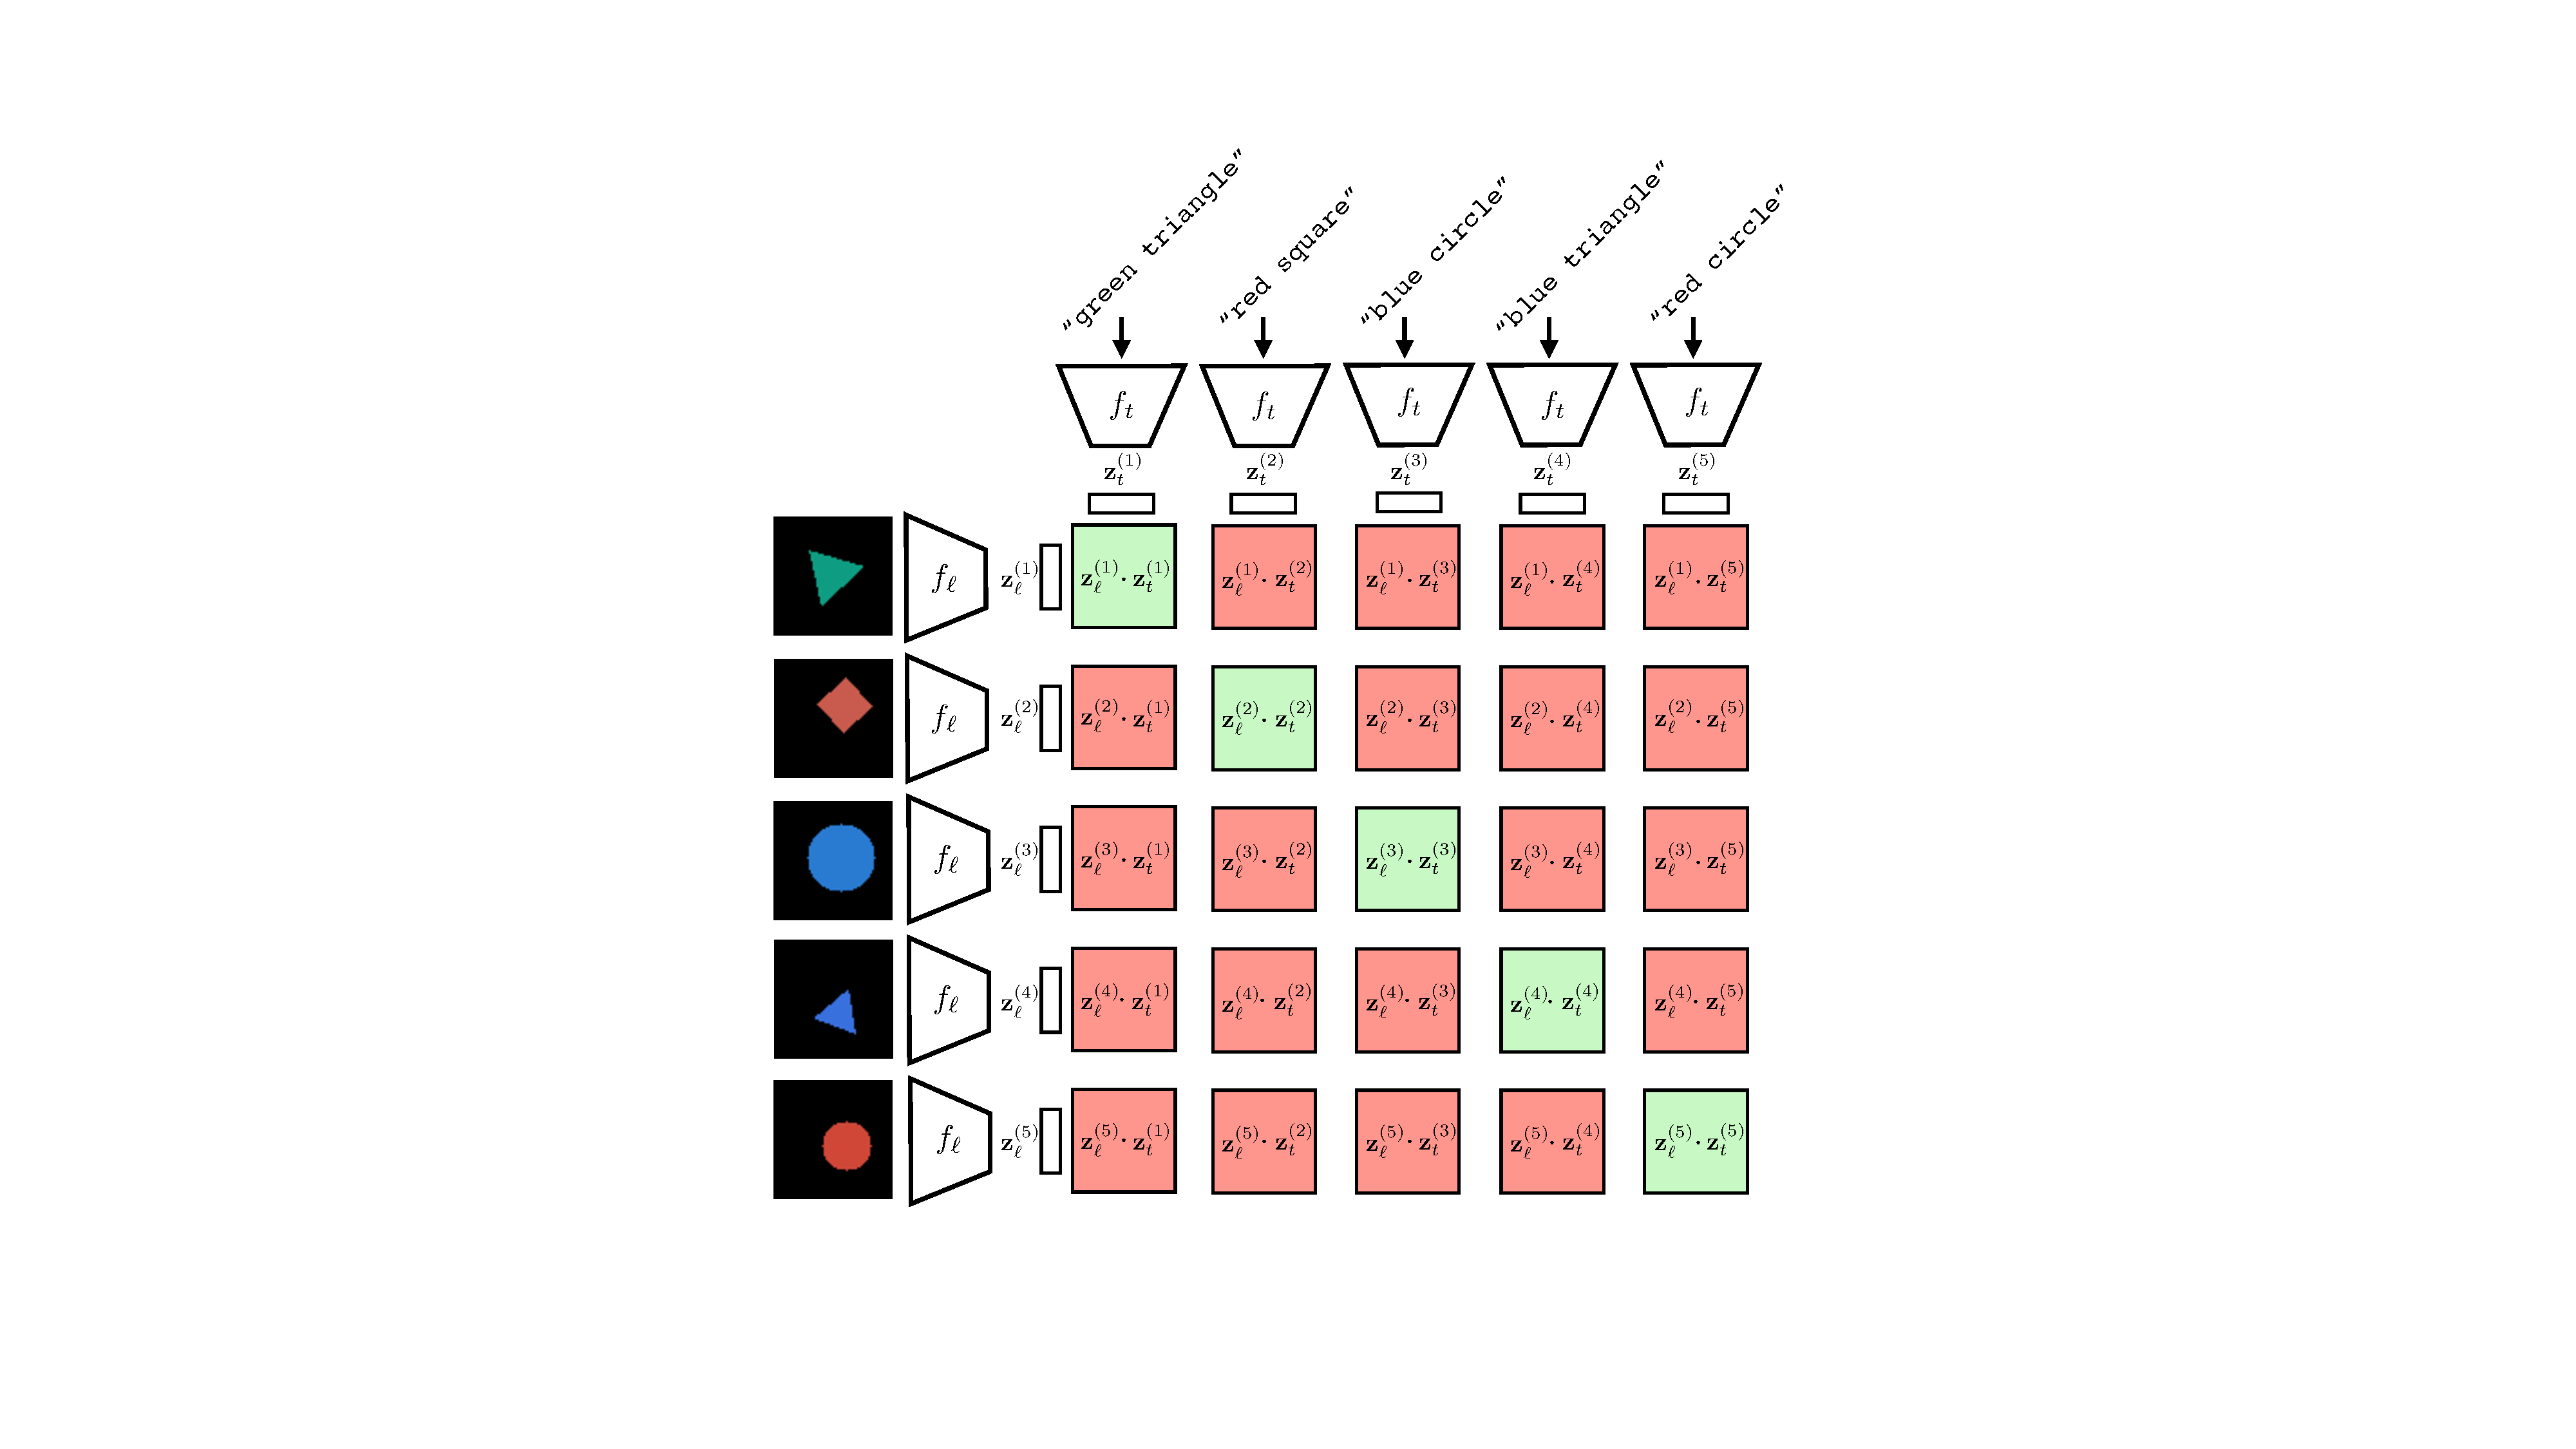
\includegraphics[width=0.85\linewidth]{figures/vision_and_language/clip_training_fig.pdf}
    }
    \caption{CLIP training for one batch of six language-image training examples. Green boxes are positive pairings (we seek to increase their value); these are the six training pairs. Red boxes are negative pairings (we seek to decrease their value); these are all other possible pairings within the batch. Inspired by figure 1 of \cite{radford2021learning}.}
    \label{fig:vision_and_language:clip_training}
\end{figure}

After training, we have a text encoder $f_t$ and an image encoder $f_\img$ that map to the same embedding space. In this space, the angle between a text embedding and an image embedding will be small if the text matches the matches. \marginnote{The dot product between unit vectors is proportional to the angle between the vectors.}[-0.7cm]
\Fig{\ref{fig:vision_and_language:clip_mapping_diagram_two_branch}} shows how a trained CLIP model maps data to embeddings. This figure is generated in the same way as \fig{\ref{fig:neural_nets:vit_mapping_plot}}: for each encoder we reduce dimensionality for visualization using \index{t-Distributed Stochastic Neighbor Embedding}\textbf{t-distributed Stochastic Neighbor Embedding} (\textbf{t-SNE})~\cite{tsne}. For the image encoder, we show the visual content using icons to reflect the color and shape depicted in the image (we previously used the same visualization in \sect{\ref{sec:representation_learning:expt_designing_embeddings_with_contrastive_learning}}). It's a bit hard to see, but one thing you can notice here is that for the image encoder, the early layers group images by color and the later layers group more by shape. The opposite is true for the text encoder. Why do you think this is? One reason may be that color is a superficial feature in pixel-space while shape requires processing to extract, but in text-space, color words and shape words are equally superficial and easy to group sentences by.
\begin{figure}[h]
    \centerline{
        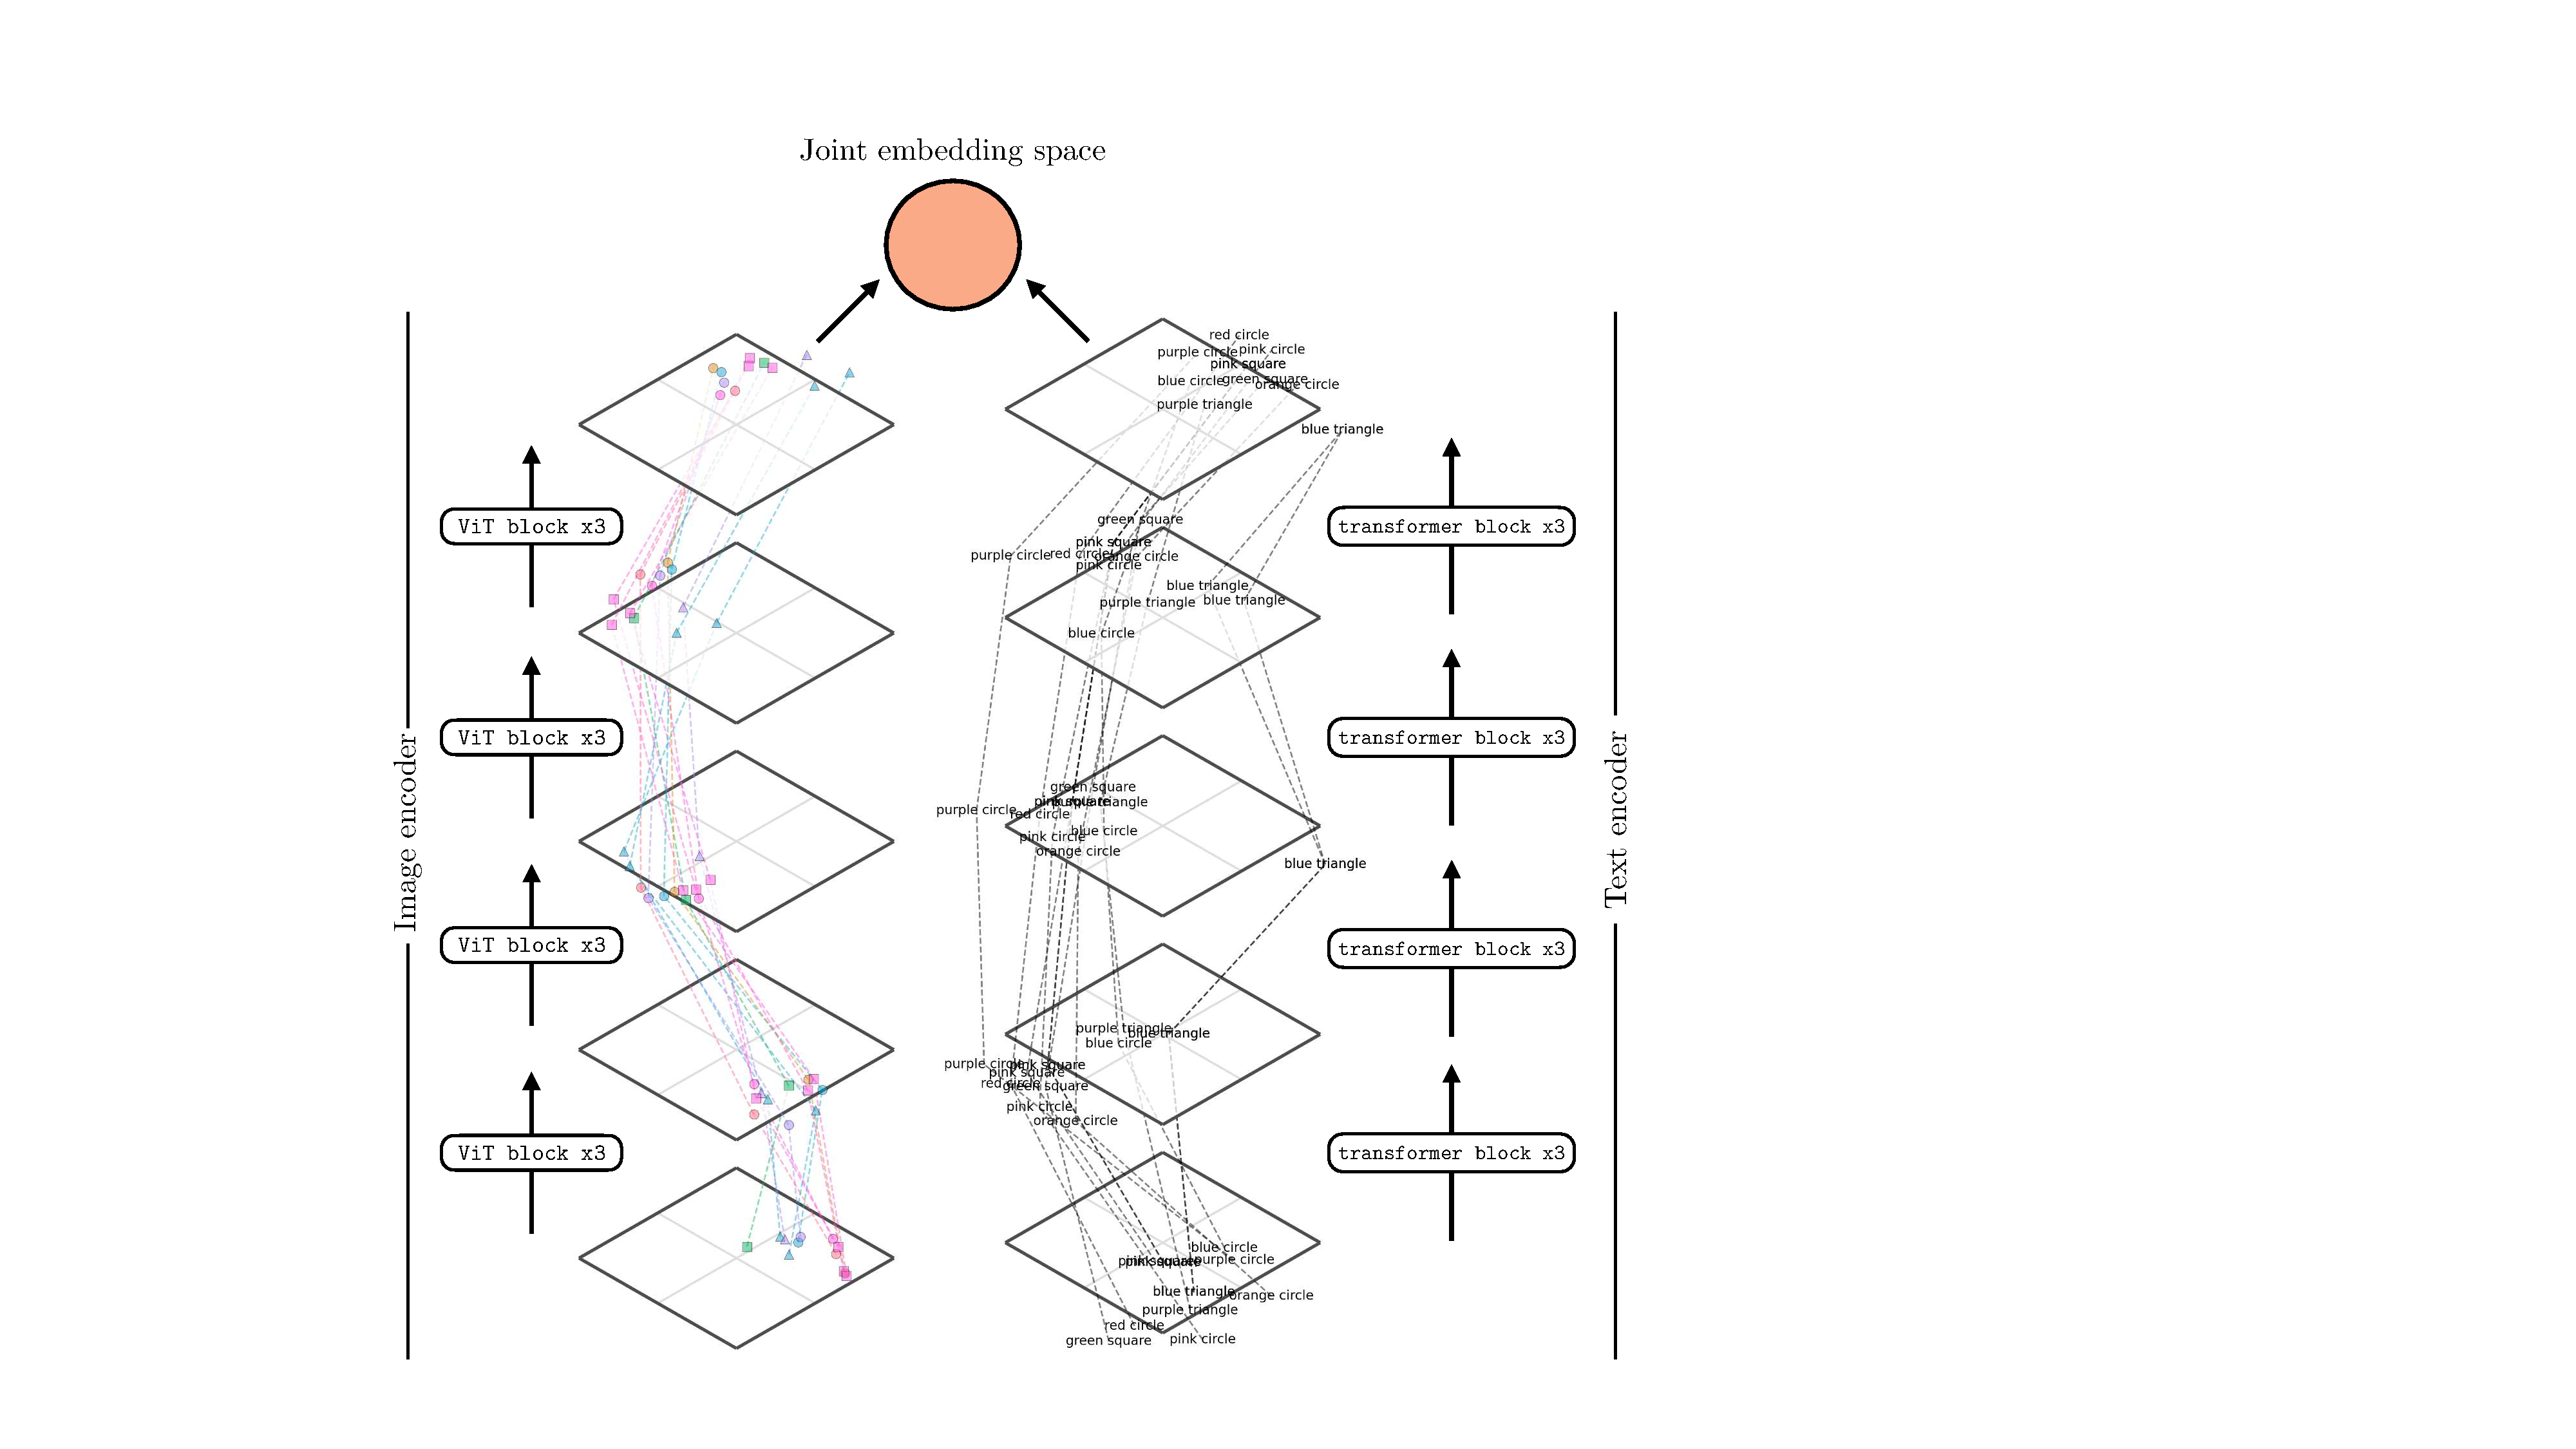
\includegraphics[width=1.0\linewidth]{figures/vision_and_language/clip_mapping_diagram_two_branch.pdf}
    }
    \caption{CLIP~\cite{radford2021learning} mapping diagram, using the same technique as described in \chap{\ref{chapter:neural_nets_as_distribution_transformers}}. To reduce dimensionality we apply t-SNE~\cite{tsne} separately for the text encoder and the image encoder. Within each encoder, we run t-SNE jointly across all shown layers.}
    \label{fig:vision_and_language:clip_mapping_diagram_two_branch}
\end{figure}

After passing the data through these two encoders, the final stage is to normalize the outputs and compute the alignment between the image and text embeddings. \Fig{\ref{fig:vision_and_language:clip_shared_embedding}} shows this last step. After normalization, all the embeddings line on the surface of a hypersphere (the circle in the figure). Notice that the text descriptions are embedded near the image embeddings (icons) that match that description. It's not perfect but note that this is partially due to limitations in the visualization, which projects the $768$-dimensional CLIP embeddings into a 2D visualization. Here we use kernel principle component analysis~\cite{scholkopf1998nonlinear} on the embeddings, with a cosine kernel, and remove the first principle component as that component codes for a global offset between the image embeddings and text embeddings.
\begin{figure}[h]
    \centerline{
        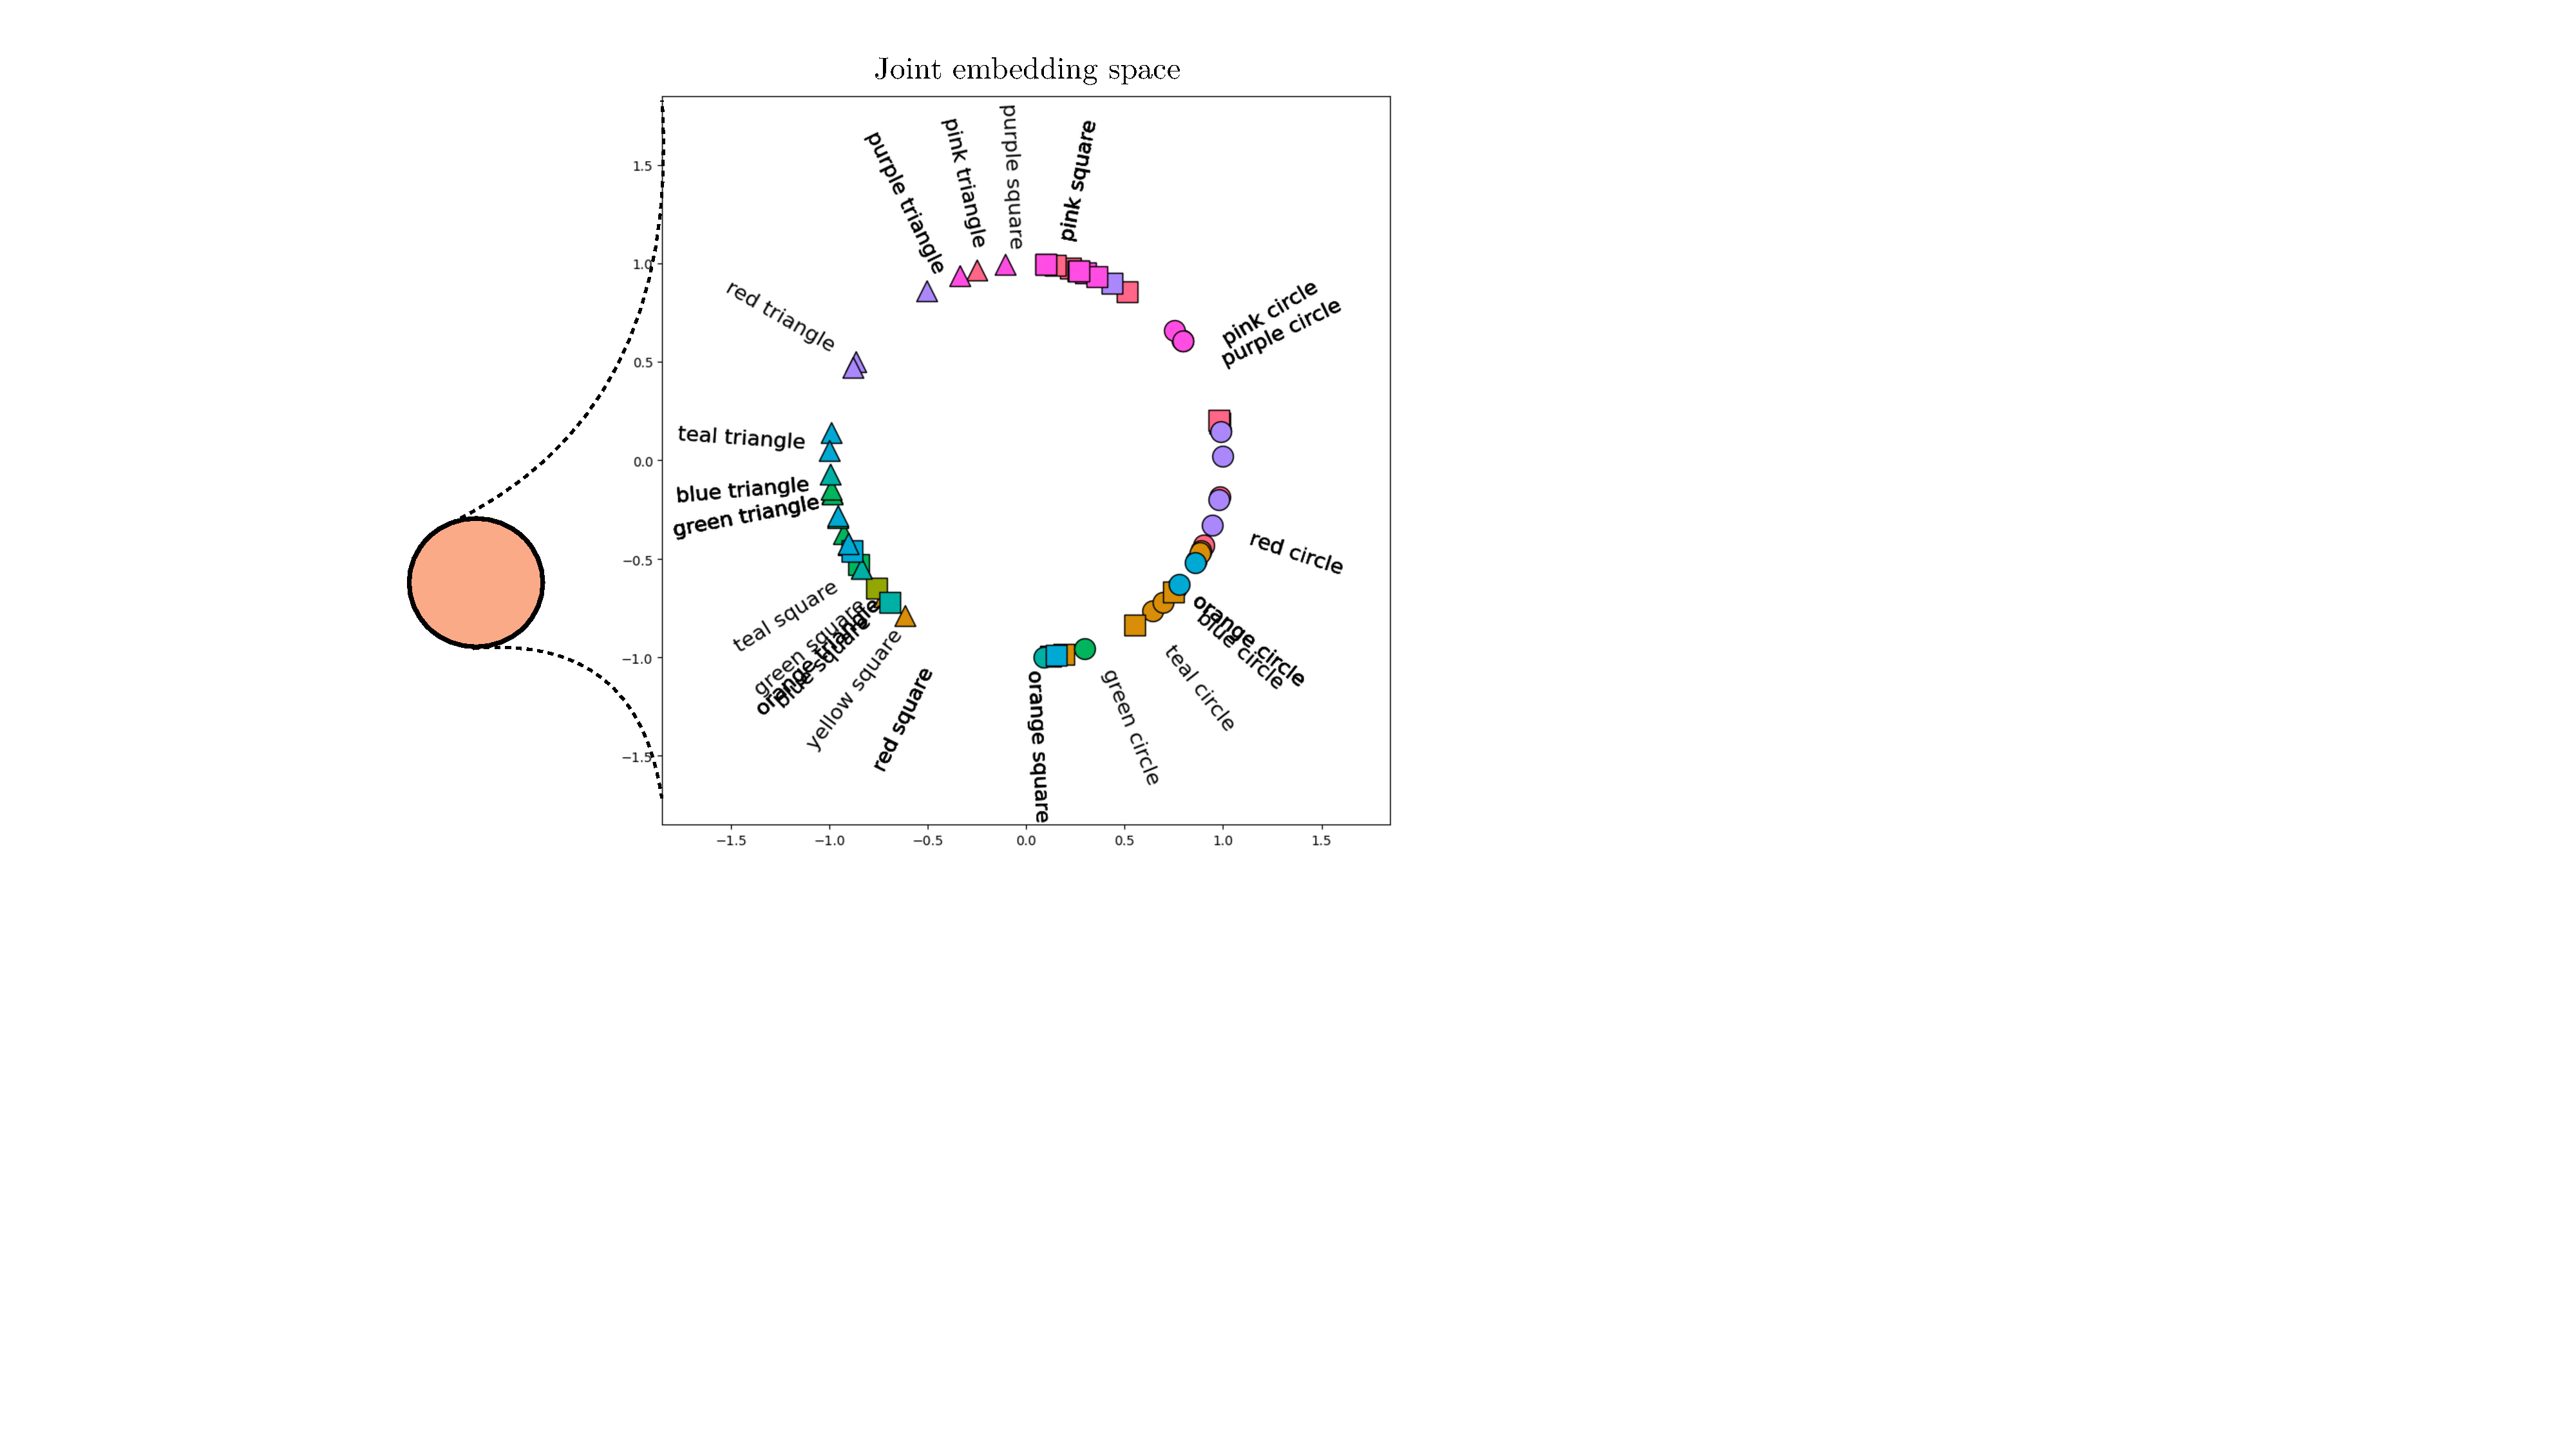
\includegraphics[width=0.8\linewidth]{figures/vision_and_language/clip_shared_embedding.pdf}}
    \caption{CLIP~\cite{radford2021learning} joint embedding.}
    \label{fig:vision_and_language:clip_shared_embedding}
\end{figure}

Using language as one of the views may seem like a minor variation on the contrastive methods we saw previously, but it's a change that opens up a lot of new possibilities. CLIP connects the domain of images to the domain of language. This means that many of the powerful abilities of language become applicable to imagery as well. One ability that the CLIP paper showcased is making a novel image classifier on the fly. With language, you can describe a new conceptual category with ease. Suppose I want a classifier to distinguish striped red circles from polka dotted green squares. These classes can be described in English just like that: ``striped red circles'' versus ``polka dotted green square.'' CLIP can then leverage this amazing ability of English to compose concepts and construct an \textit{image} classifier for these two concepts.

Here's how it works. Given a set of sentences $\{\mathbf{t}^{a}, \mathbf{t}^{b}, \ldots\}$ that describe images of classes $a$, $b$, and so on,
\begin{enumerate}
    \item Embed each sentence into a $\mathbf{z}$-vector, $\mathbf{z}_t^{a} = f_t(\mathbf{t}^{a}), \mathbf{z}_t^{b} = f_t(\mathbf{t}^{a}),$ and so on.
    \item Embed your query image into a $\mathbf{z}$-vector, $\mathbf{z}_{\img}^{q} = f_{\img}(\boldimg^{q})$.
    \item See which sentence embedding is closest to your image embedding; that's the predicted class.
\end{enumerate}
These steps are visualized in \fig{\ref{fig:vision_and_language:clip_inference}}. The green outlined dot product is the highest, indicating that the query image will be classified as class $a$, which is defined as ``striped red circles.''
\begin{figure}[h]
    \centerline{
        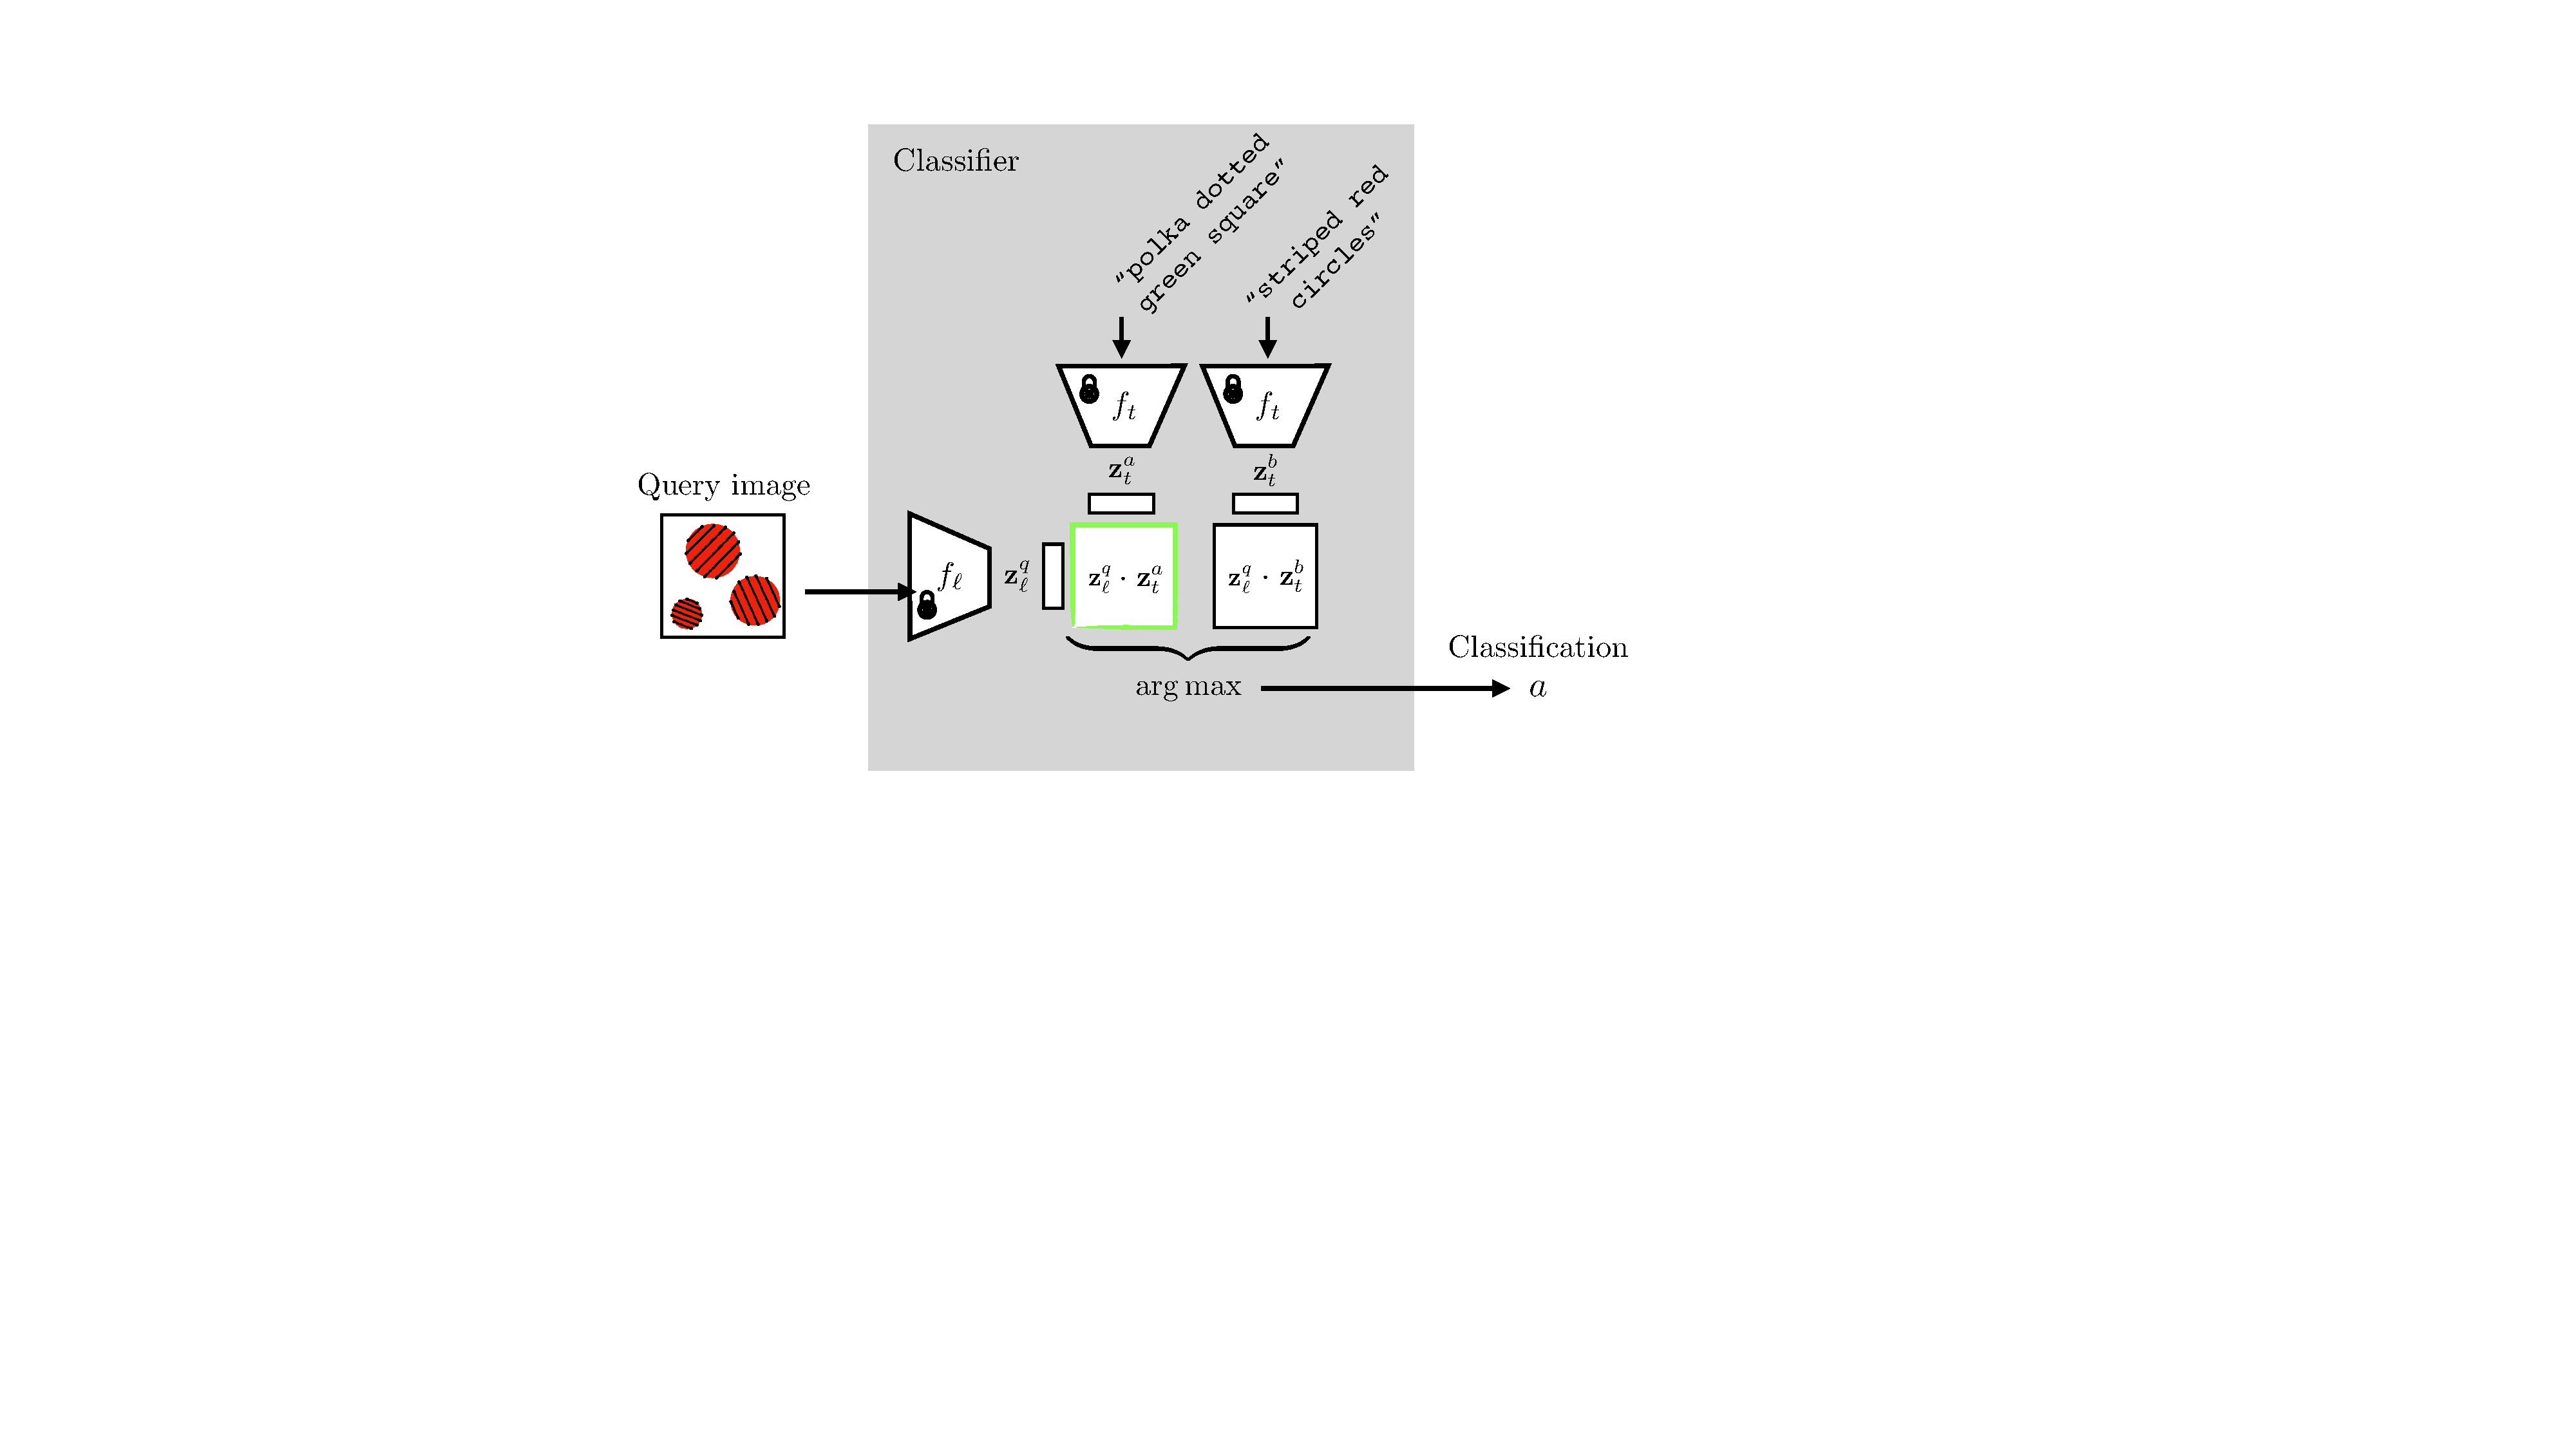
\includegraphics[width=0.75\linewidth]{figures/vision_and_language/clip_inference_fig.pdf}
    }
    \caption{Making a ``striped red circles'' (class $a$) versus ``polka dotted green square'' (class $b$) classifier using a trained CLIP. The CLIP model parameters are frozen and not updated. Instead the classifier is constructed by embedding the text describing to the two classes and seeing which is closer to the embedding of the query image. Inspired by figure 1 of \cite{radford2021learning}.}
    \label{fig:vision_and_language:clip_inference}
\end{figure}
% \begin{figure}[h]
%     \centerline{
%         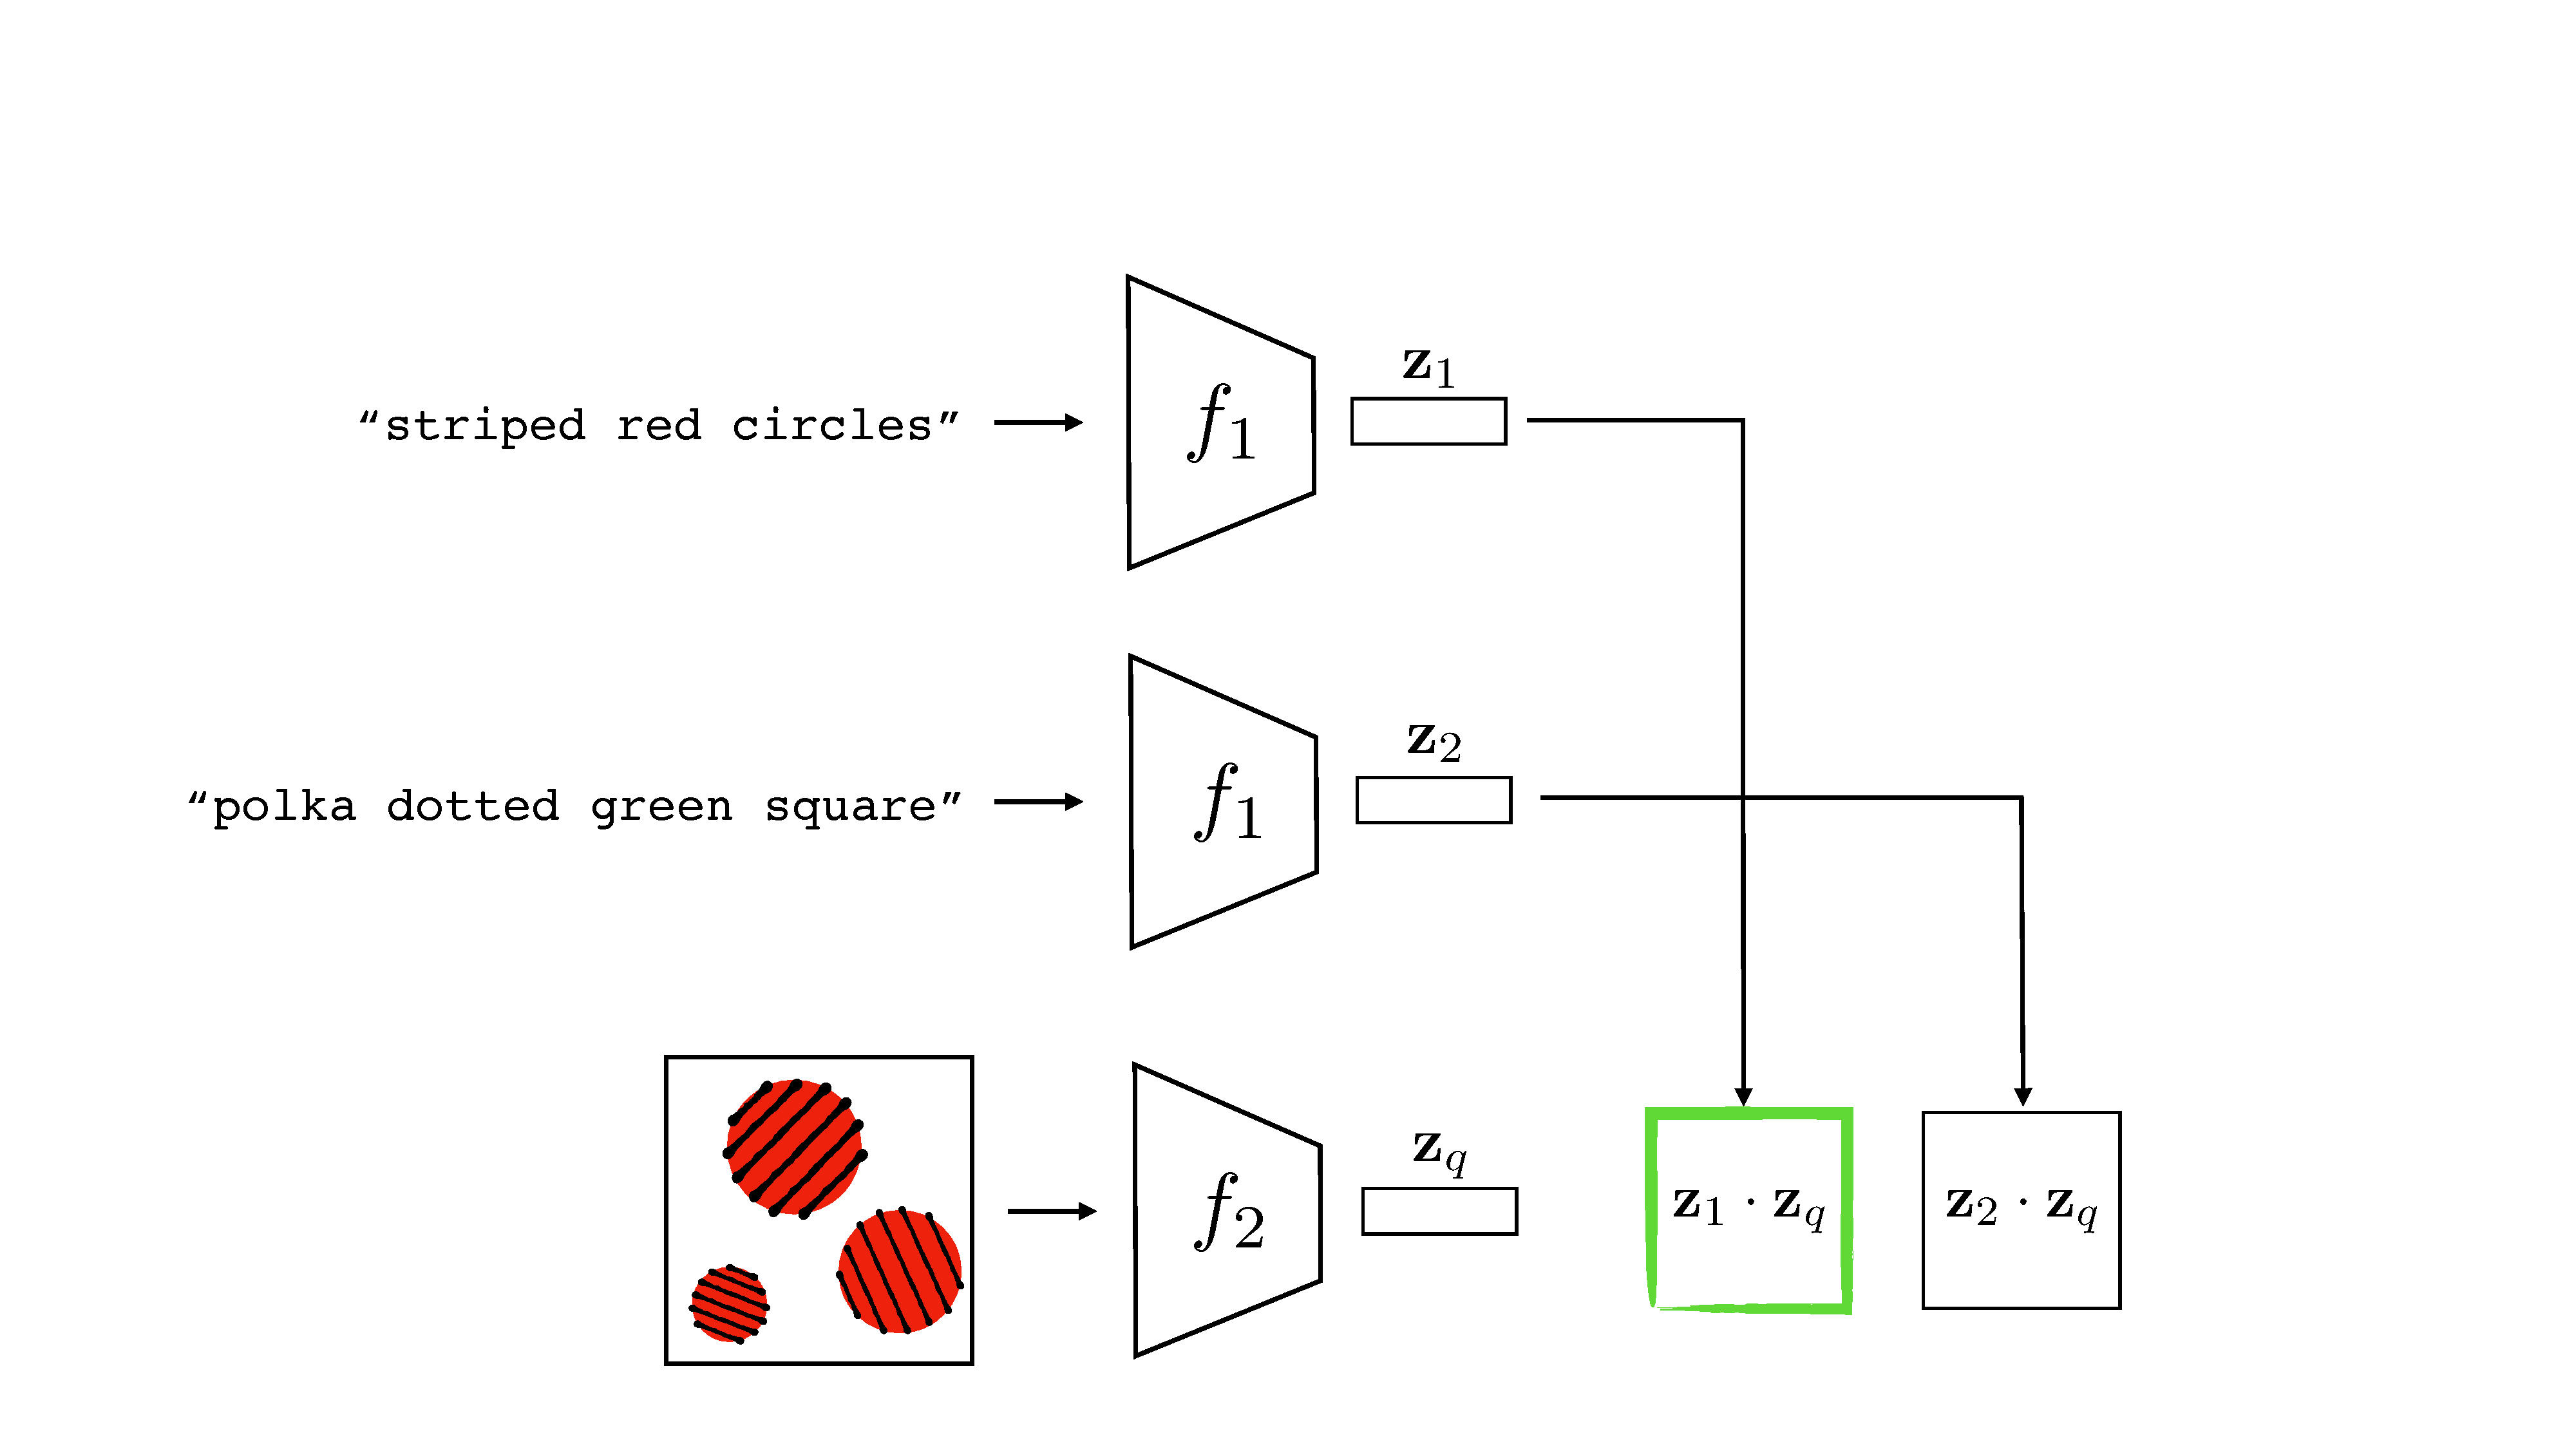
\includegraphics[width=0.8\linewidth]{figures/representation_learning/clip_schematic.pdf}
%         \caption{CLIP~\cite{radford2021learning} can construct a classifier on-the-fly just by embedding the natural language descriptions of two classes.}
%         \label{fig:representation_learning:clip_schematic}
%     }
% \end{figure}
\Fig{\ref{fig:vision_and_language:clip_clocks}} gives more examples of creating custom binary classifiers in this way. The two classes are described by two text strings (``triangle'' versus ``cricle''; ``purple'' versus ``teal''; and ``arrowhead'' versus ``ball''). The embeddings of the text descriptions are the red and green vectors. The classifier simply checks where an image embedding is closer, in angular distance, to the red vector or the green vector. This approach isn't limited to binary classification: you can add more text vectors to partition the space in more ways.

\begin{figure}[h]
    \centerline{
        \begin{subfigure}{0.25\textwidth}
            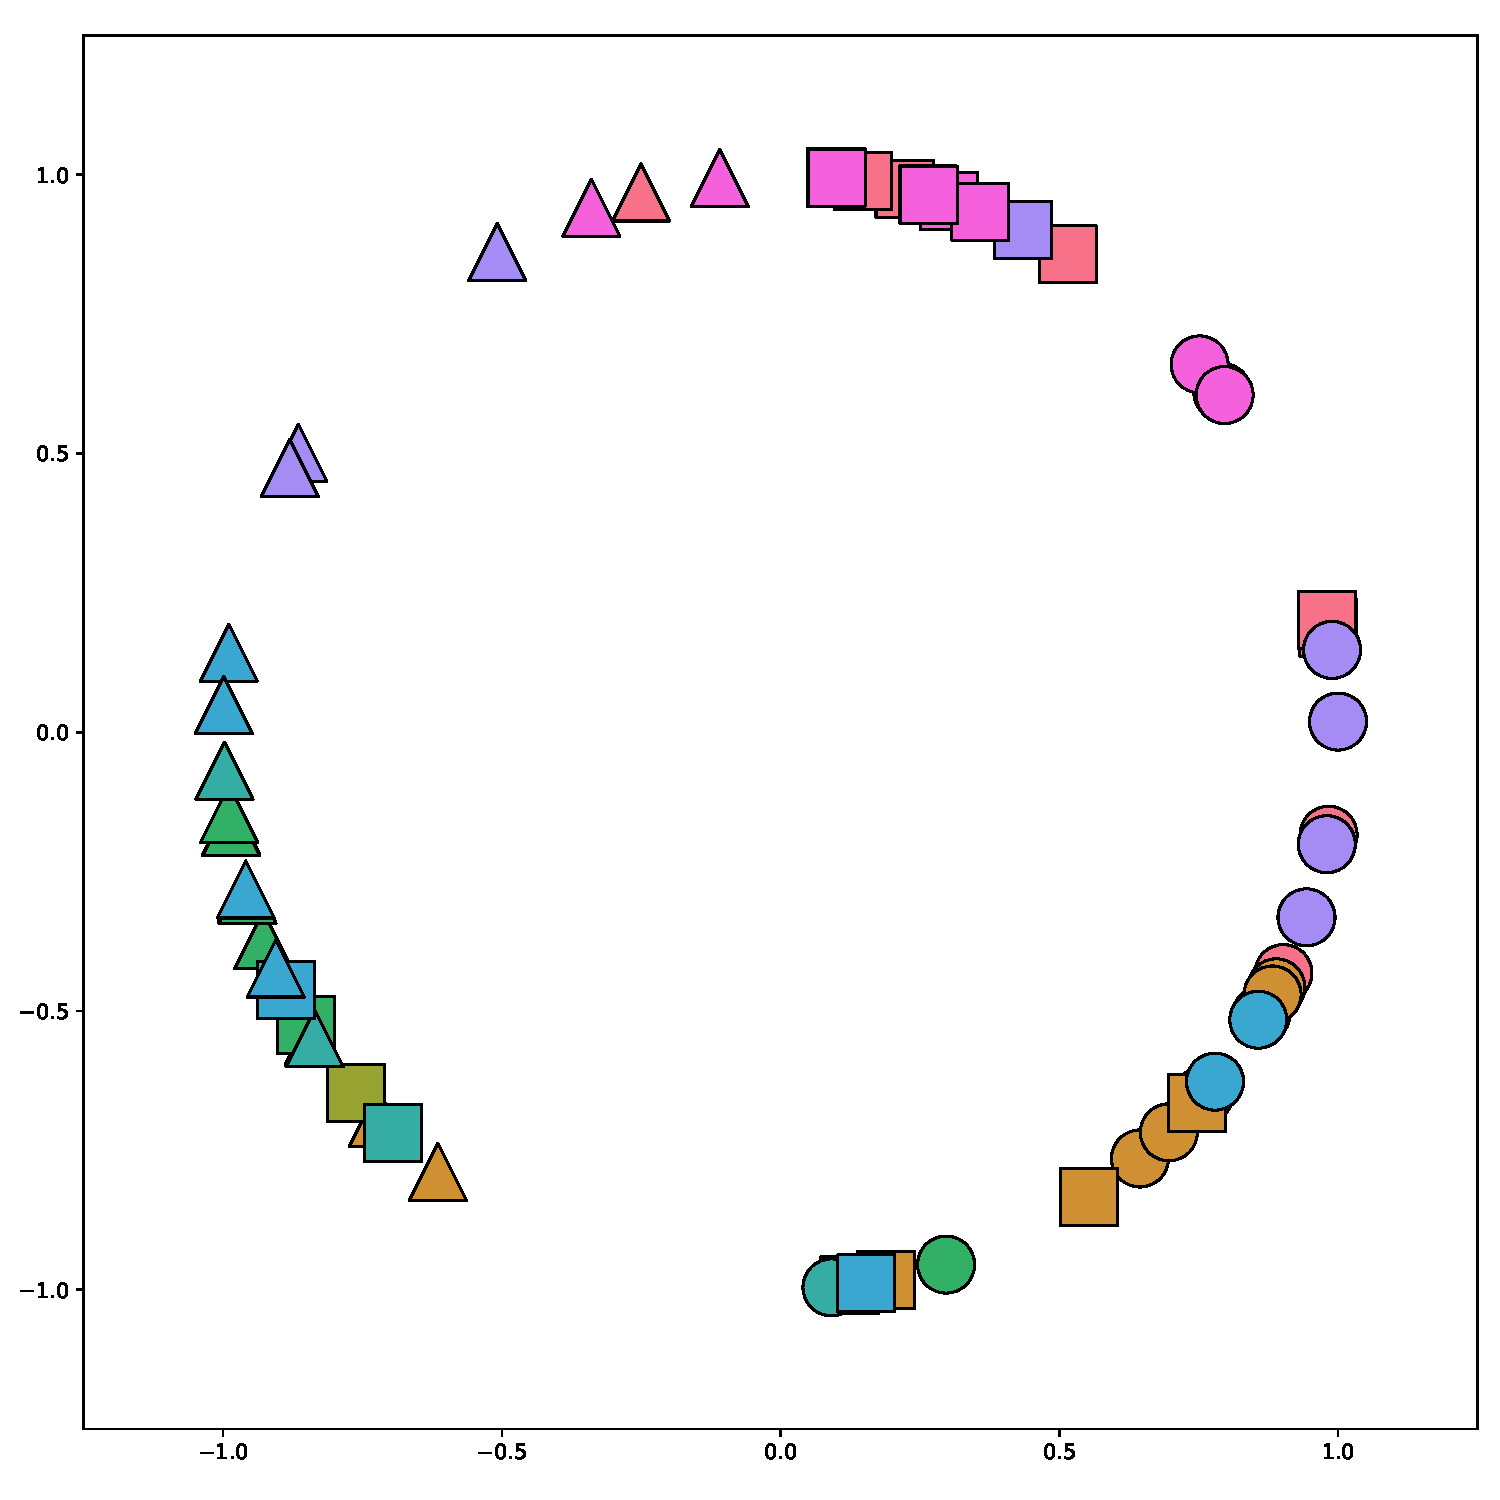
\includegraphics[width=\linewidth]{figures/vision_and_language/clip_clocks/joint_embedding.pdf}
            \caption*{(a)}
        \end{subfigure}%
        \hspace*{\fill}   % maximize separation between the subfigure
        \begin{subfigure}{0.25\textwidth}
            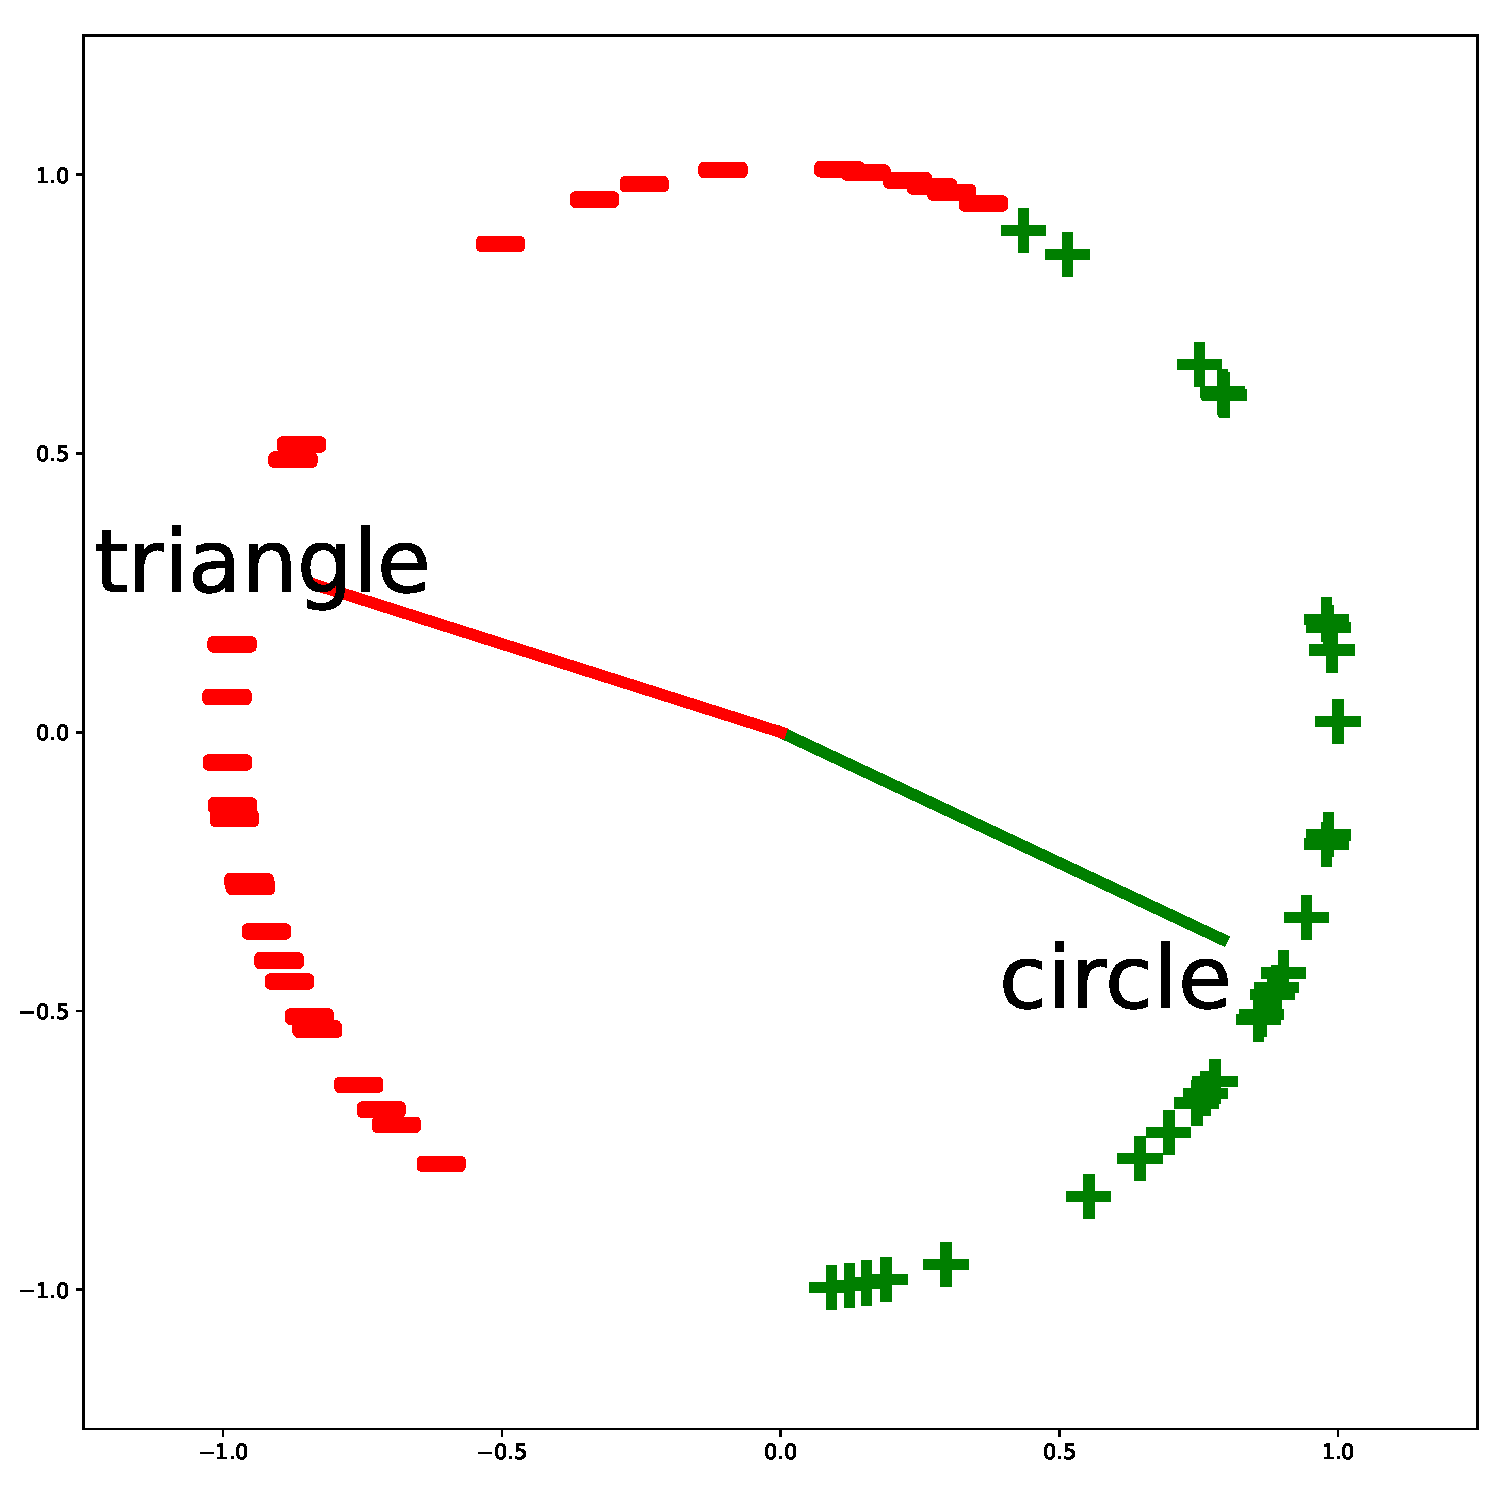
\includegraphics[width=\linewidth]{figures/vision_and_language/clip_clocks/circle_triangle.pdf}
            \caption*{(b)}
        \end{subfigure}%
        \hspace*{\fill}   % maximize separation between the subfigure
        \begin{subfigure}{0.25\textwidth}
            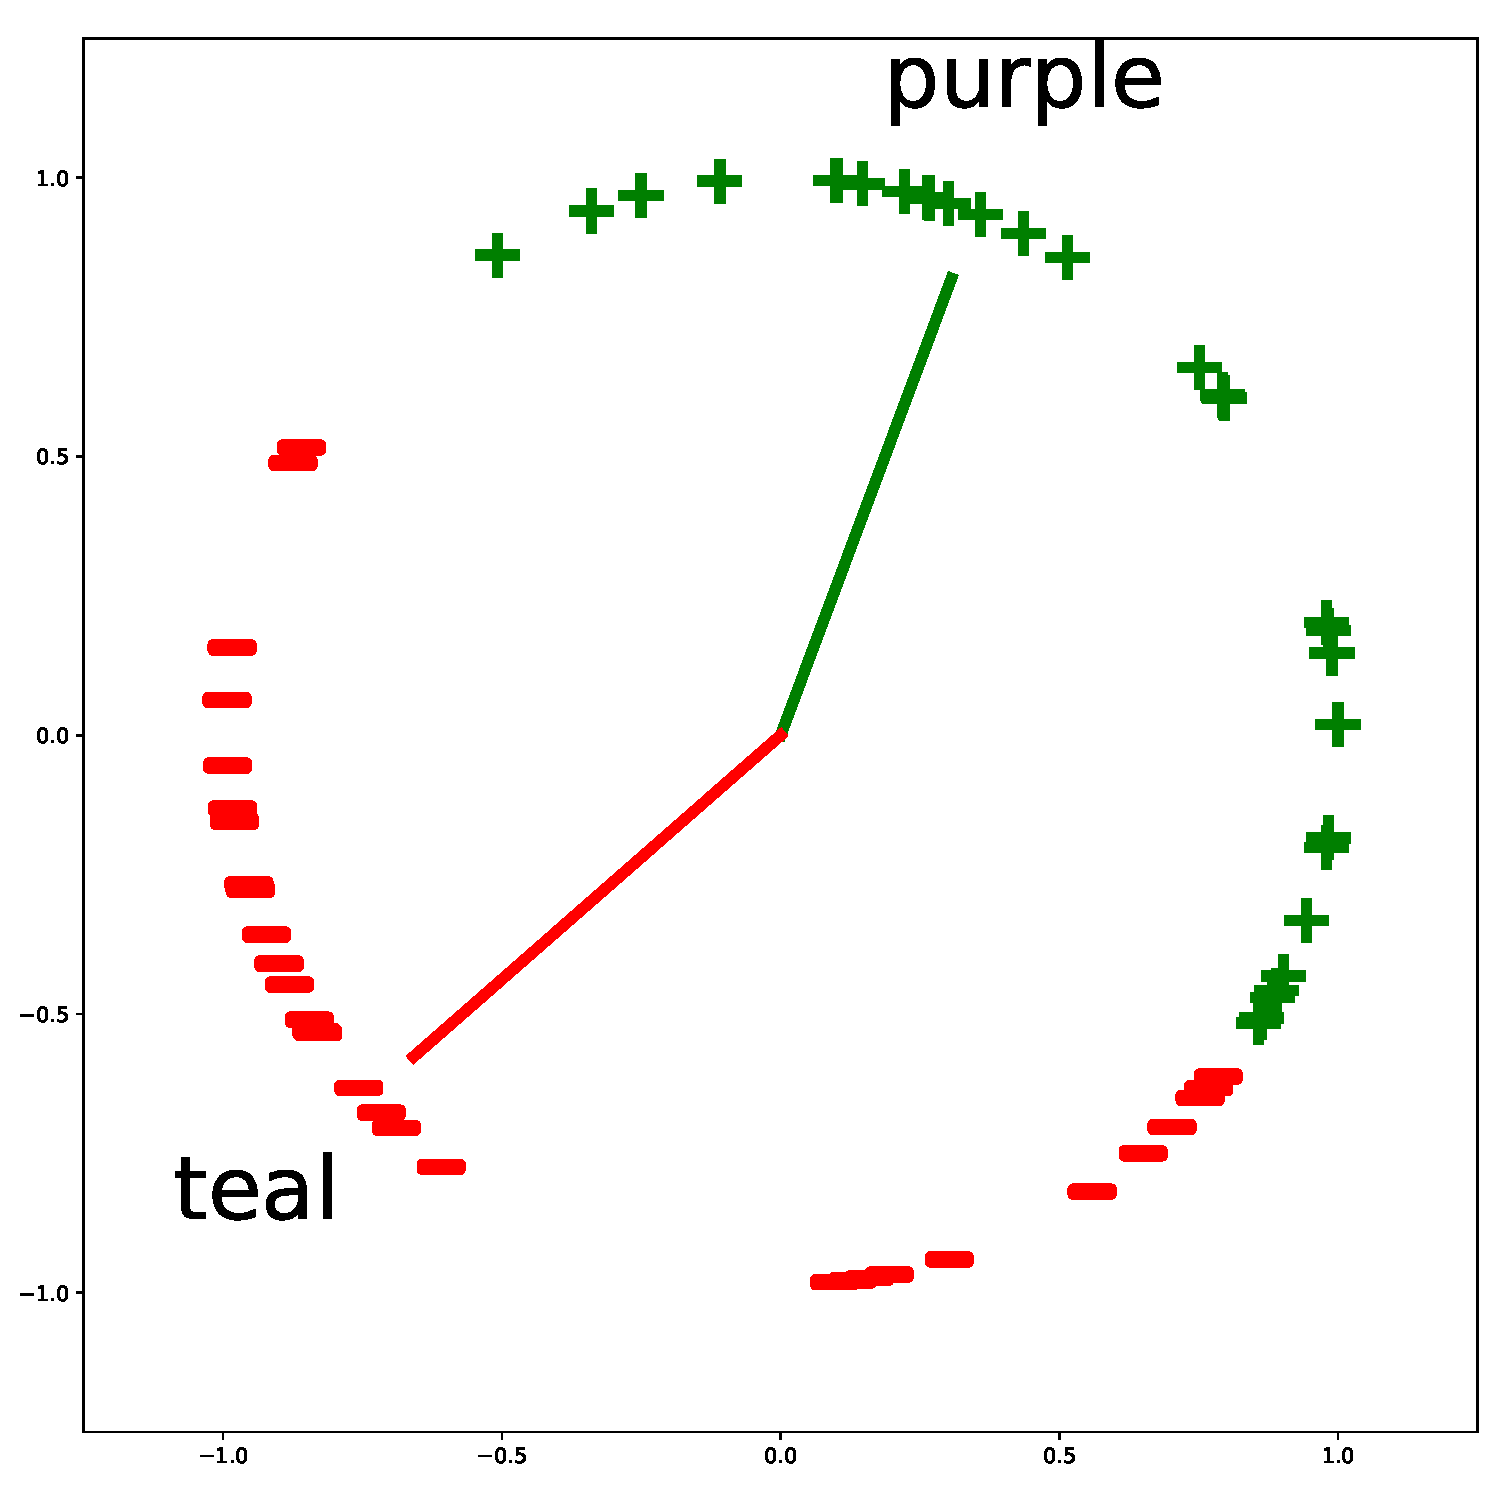
\includegraphics[width=\linewidth]{figures/vision_and_language/clip_clocks/purple_teal.pdf}
            \caption*{(c)}
        \end{subfigure}%
        \hspace*{\fill}   % maximize separation between the subfigure
        \begin{subfigure}{0.25\textwidth}
            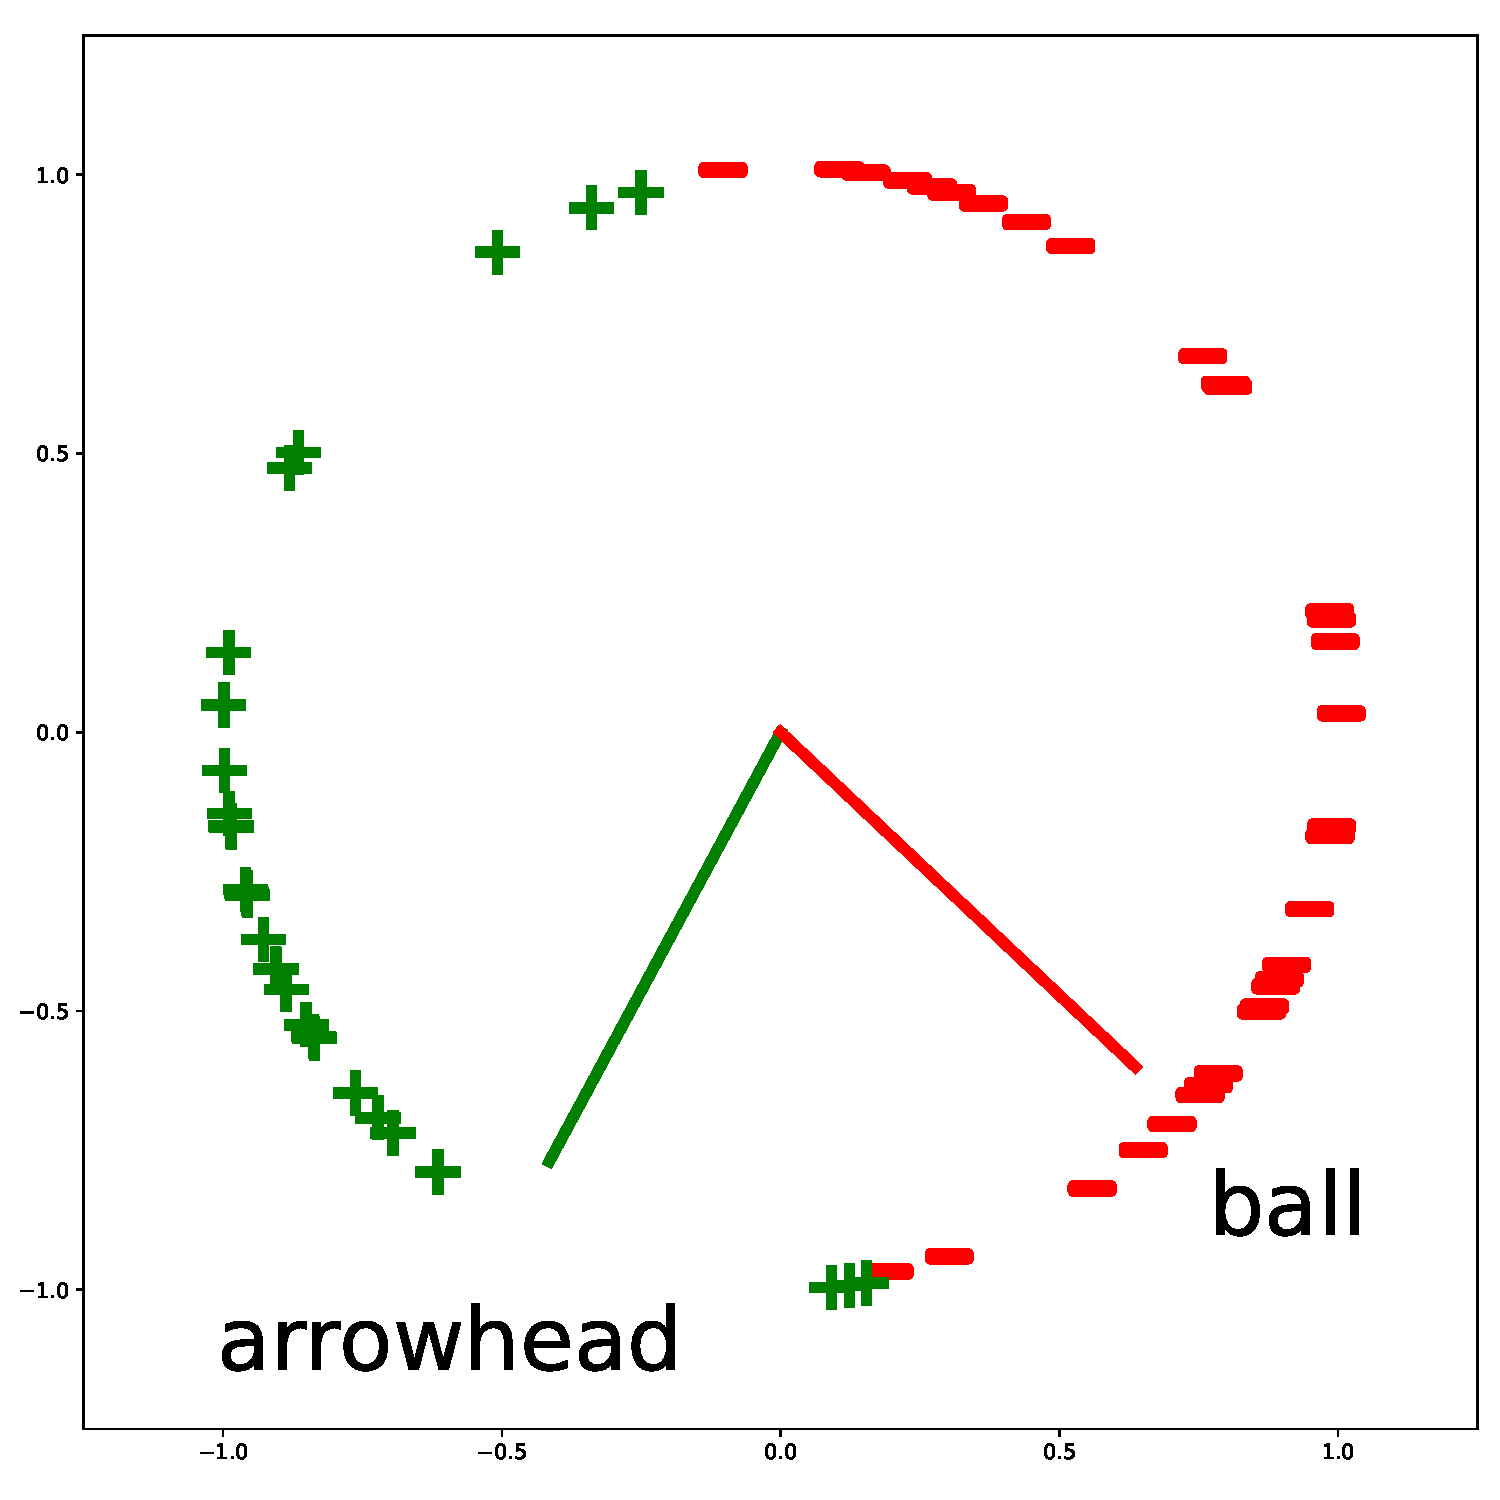
\includegraphics[width=\linewidth]{figures/vision_and_language/clip_clocks/arrowhead_ball.pdf}
            \caption*{(d)}
        \end{subfigure}%
    }
    \caption{Making custom classifiers using CLIP. (a) Image embeddings in joint embedding space, (b) triangle-circle classifier, (c) purple-teal classifier, and (d) arrowhead-ball classifier. It's a bit like a modern astrolabe where you turn dials to read off the prediction of interest.}
    \label{fig:vision_and_language:clip_clocks}
\end{figure}

\section{Translating between Images and Text}

In \chap{\ref{chapter:conditional_generative_models}}, we saw how to translate between different image domains. Could we be even more ambitious and translate between entirely different data \textit{modalities}? It turns out that this is indeed possible and is an area of growing interest. For any type of data X, and any other type Y, there is, increasingly, a method X2Y (and Y2X) that translates between these two data types. Go ahead and pick your favorite data types—X,Y could be images and sounds, music and lyrics, amino acid sequences and protein geometry—then Google ``X to Y with a deep net'' and you will probably find some interesting work that addresses this problem. X2Y systems are powerful because they forge links between disparate domains of knowledge, allowing tools and discoveries from one domain to become applicable to other linked domains.

One approach to solving X-to-Y translation problems is do it in a modular fashion by hooking up an \textit{encoder} for domain X to a decoder for domain Y. This approach is popular because powerful encoder and decoder architectures, and pretrained models, exist for many domains. If we have an encoder $f: \mathcal{X} \rightarrow \mathcal{Z}$ and a decoder $g: \mathcal{Z} \rightarrow \mathcal{Y}$, then we can create a translator simply by function composition, $g \circ f$.

Of course, the output of our encoder might not be interpretable as a proper input to the decoder we selected. For example, suppose $f$ is a text encoder and $g$ is an image decoder and we have $\boldimg = g(f(\mathbf{t}))$, where $\boldimg$ is a generated image from the text input $\mathbf{t}$. Then nothing guarantees that $\boldimg$ semantically matches $\mathbf{t}$.

To \textit{align} the encoder and decoder we can follow several strategies. One is to simply finetune $g \circ f$ on paired examples of the target translation problem, $\{\mathbf{t}^{(i)}, \boldimg^{(i)}\}_{i=1}^N$. Another option is to freeze $f$ and $g$ and instead train a translation function in latent space, $h: \mathcal{Z} \rightarrow \mathcal{Z}$, so that $g \circ h \circ f$ correctly maps each training point $\mathbf{t}^{(i)}$ to the target output $\boldimg^{(i)}$. See \cite{rombach2022high} for an example of this latter option.

In the next sections, we will look at a few specific architectures for solving this problem of text-to-image translation as well as the reverse, image-to-text.


% \begin{enumerate}
%     \item Train an encoder for X, $f: \mathcal{X} \rightarrow \mathcal{Z}$.
%     \item Train a decoder for Y, $g: \mathcal{Z} \rightarrow \mathcal{Y}$.
%     \item Train a translator in latent space, $h: \mathcal{Z} \rightarrow \mathcal{Z}$.
% \end{enumerate}
%The first step can be achieved with any kind of representation learner, such as an autoencoder or a contrastive learner. The second step can be achieved with any kind of generator, such as a diffusion model or a GAN. The final step aligns the $z$-space of the two domains. It makes it so that the proper item in X maps to proper item in Y. This final step requires paired data whereas the first two steps do not.

%Many models take this modular approach.

%It is also possible to train X2Y models end-to-end using any kind of conditional generative model, including all the types we saw in \chap{\ref{chapter:conditional_generative_models}}.


\subsection{Text-to-Image}
%It's also possible to do translation in the opposite direction: text-to-image.
\index{Text-to-image}

One amazing ability of modern generative models is to synthesize an image just from a text description, a problem called \textbf{text-to-image}. This can be achieved using any of the conditional generative models we saw in \chap{\ref{chapter:conditional_generative_models}}. We simply have to find an effective way to use text as the conditioning information to these models. \Fig{\ref{fig:vision_and_language:text2im_schematic_mapping}} shows how this problem looks as a mapping from the space of text to the space of images:
\begin{figure}[h]
    \centerline{
        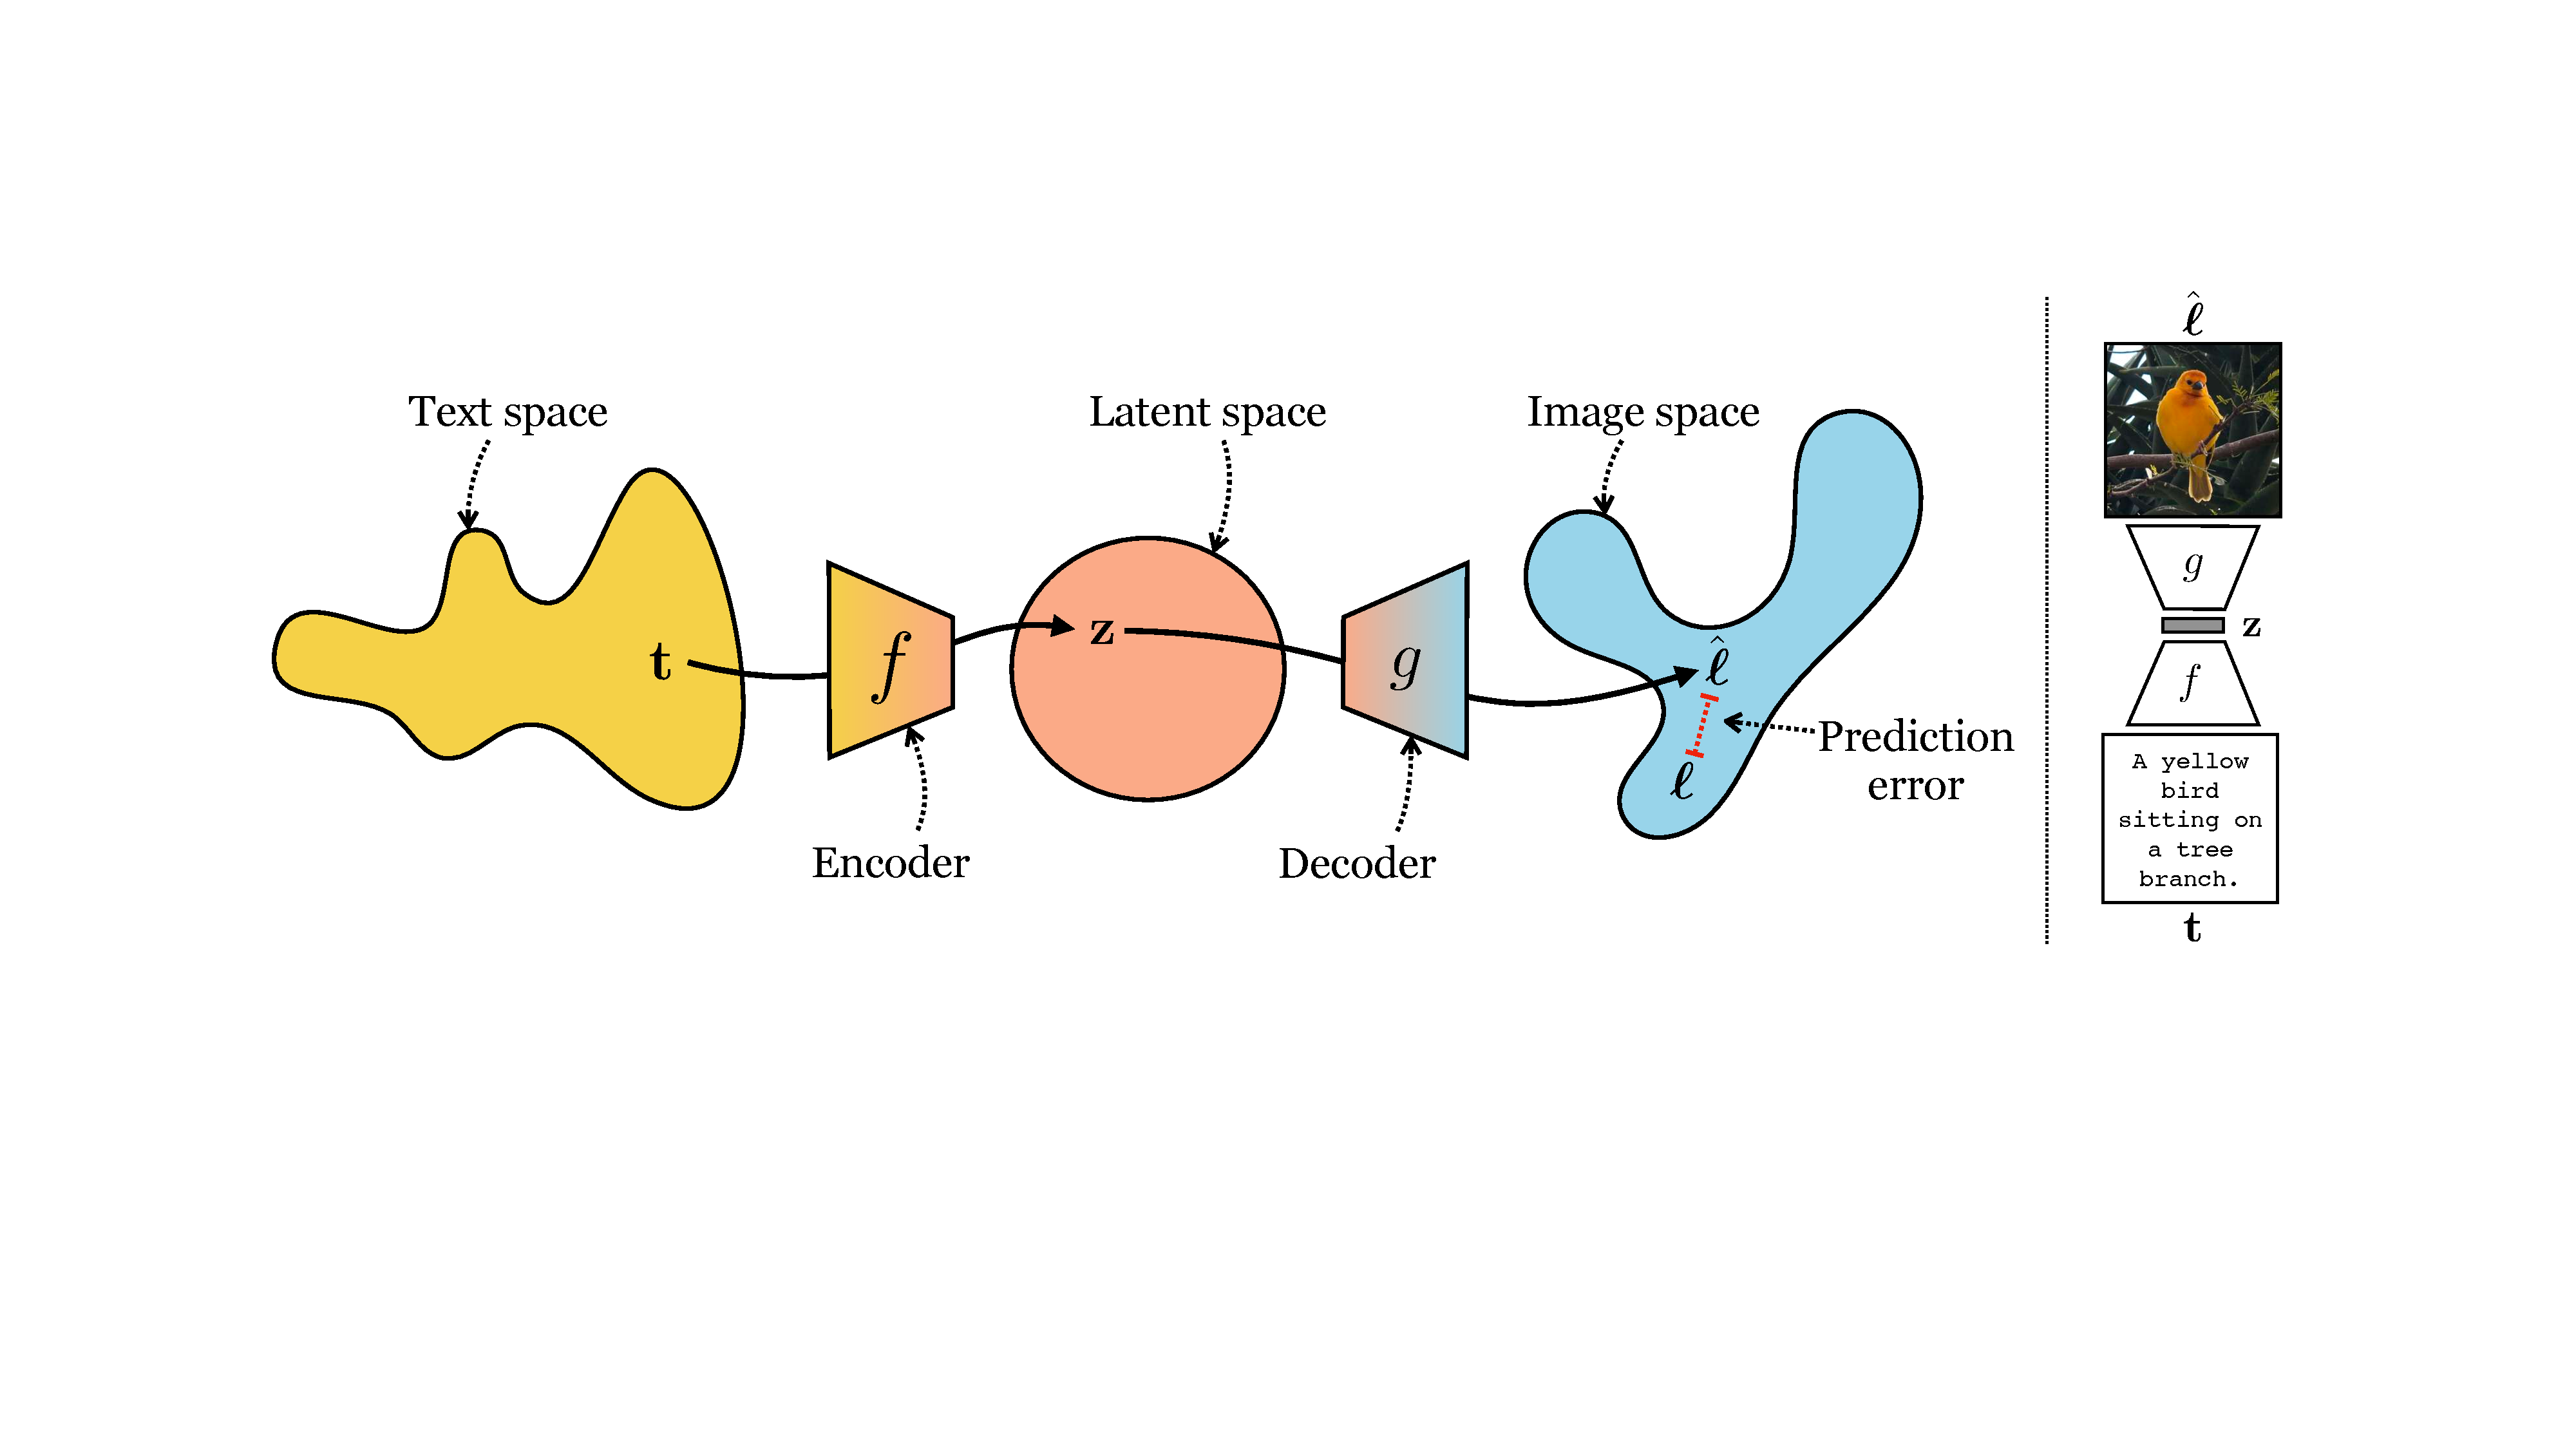
\includegraphics[width=1.0\linewidth]{figures/vision_and_language/text2im_schematic_mapping.pdf}}
    \caption{Text-to-image.}
    \label{fig:vision_and_language:text2im_schematic_mapping}
\end{figure}

On the right is an example of such a system translating input text $\mathbf{t}$ to an output image $\hat{\boldimg}$ that matches what the text describes. Recall the similar diagrams in the chapters on representation learning and generative modeling and think about how they relate (see \figs{\ref{fig:representation_learning:autoencoder_diagram}} and \ref{fig:generative_modeling_and_representation_learning:genrep_schematic}). This new problem is not so different from what we have seen before!

Now let's build some concrete architectures to solve this mapping. We will start with a conditional variational autoencoder (cVAE; \sect{\ref{sec:conditional_generative_models:cVAE}}). This was the architecture used by the DALL-E 1 model~\cite{dalle1}, which was one of the first text-to-image models that caught the public's imagination.

A cVAE for text-to-image can be trained just like a regular cVAE; the special thing is just that the encoder is a text encoder, that is, a neural net that maps from text to a vector embedding. \Fig{\ref{fig:vision_and_language:text2im_VAE_training}} shows what the training looks like; it's conceptually the same as \fig{\ref{fig:conditional_generative_models:cVAE_ball_bouncing_example_nets}}, which we saw previously.
\begin{figure}[h!]
    \centerline{
        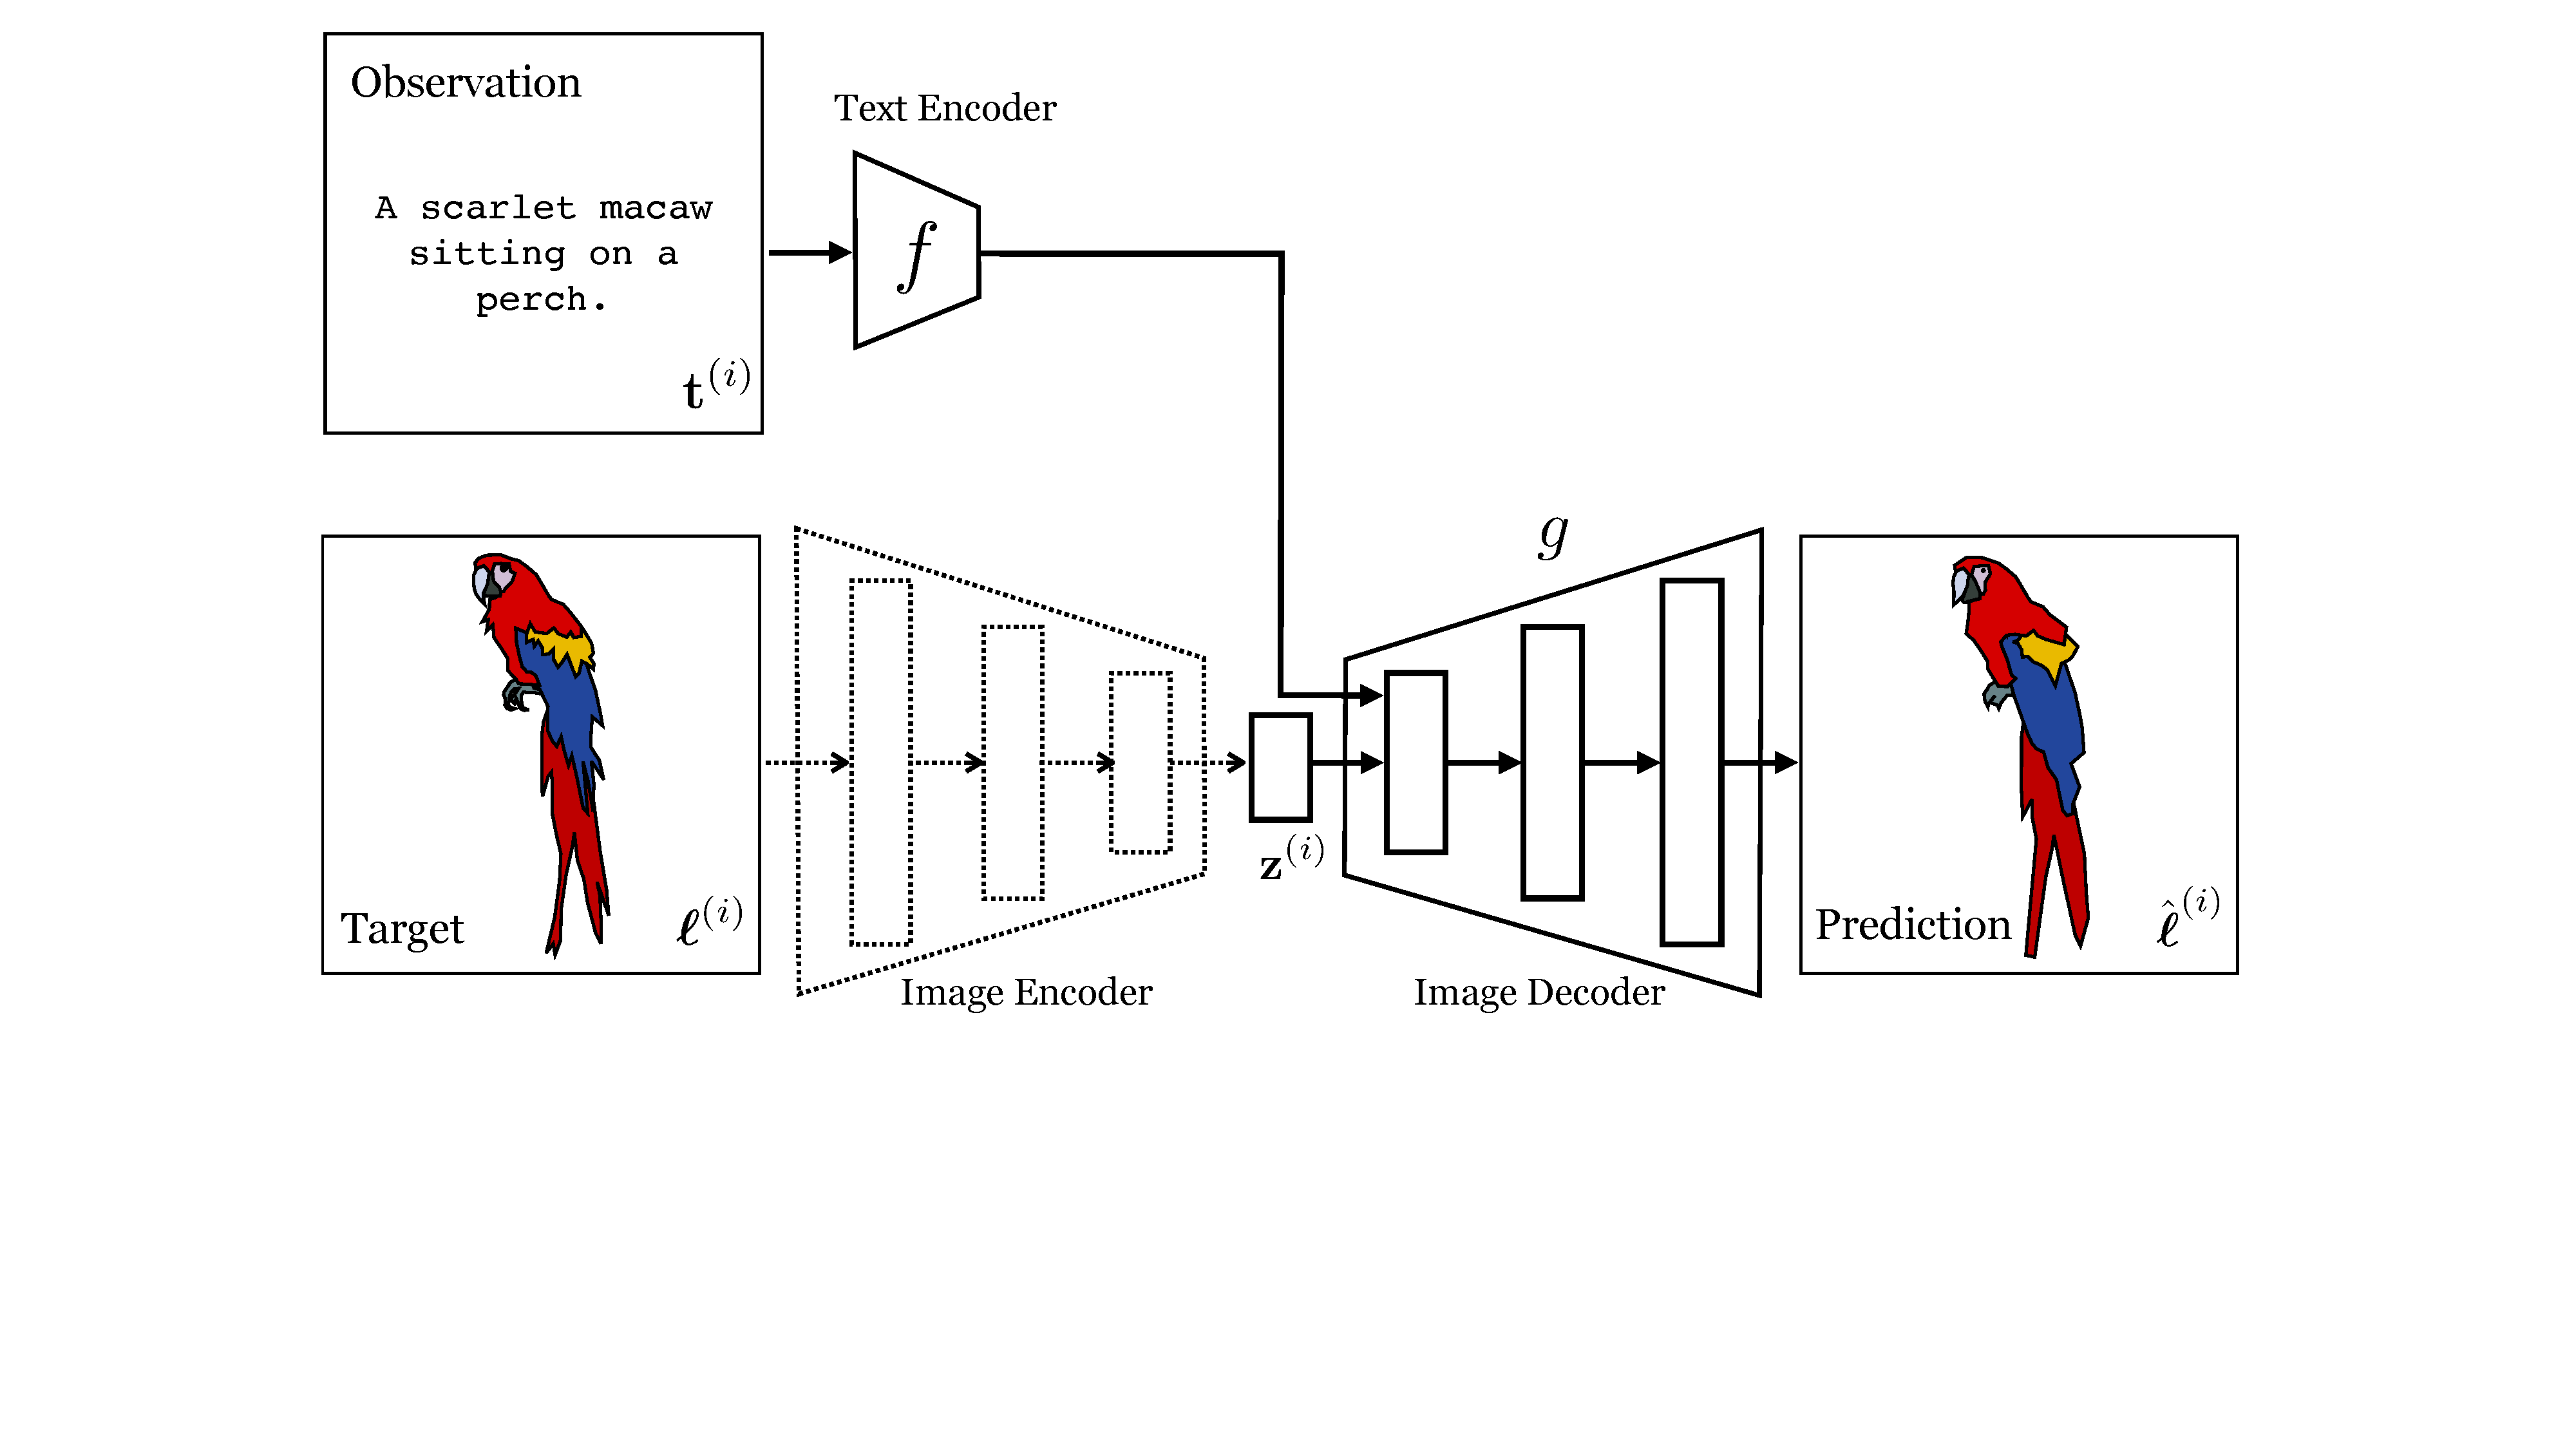
\includegraphics[width=1.0\linewidth]{./figures/vision_and_language/text2im_VAE_training.pdf}
    }
    \caption{Training a cVAE to perform text-to-image. The dotted lines indicate that the image encoder is only used during training; at test time, usage follows the solid path. In this cartoon we draw the output as slightly distorted to reflect that the autoencoder path might not be able to perfectly reconstruct the input.}
    \label{fig:vision_and_language:text2im_VAE_training}
\end{figure}

After training this model, we can sample from it by simply discarding the image encoder and instead inputting a random Gaussian vector to the decoder, in addition to providing the decoder with the text embedding. \Fig{\ref{fig:vision_and_language:text2im_VAE_sampling}} shows how to sample an image in this way.

This is how text-to-image generation can be done with a cVAE. We could perform the same exercise for any conditional generative model. Let's do one more, a conditional diffusion model. This is the approach followed by the second version of the DALL-E system, DALL-E 2~\cite{ramesh2022hierarchical}, as well as other popular systems like the one described in \cite{rombach2022high}. The difficulty we will focus on here is as follows: how do you most effectively insert the text embeddings into the the decoder, so that it can make best use of this information? \Fig{\ref{fig:vision_and_language:text2im_diffusion_model}} shows one way to do this, which is roughly how it is done in \cite{rombach2022high}: we insert text embedding vectors into each denoising U-Net, and even into multiple layers of each U-Net. This makes it very easy for the diffusion model to condition all of its decisions on the text information.
\begin{figure}[h!]
    \centerline{
        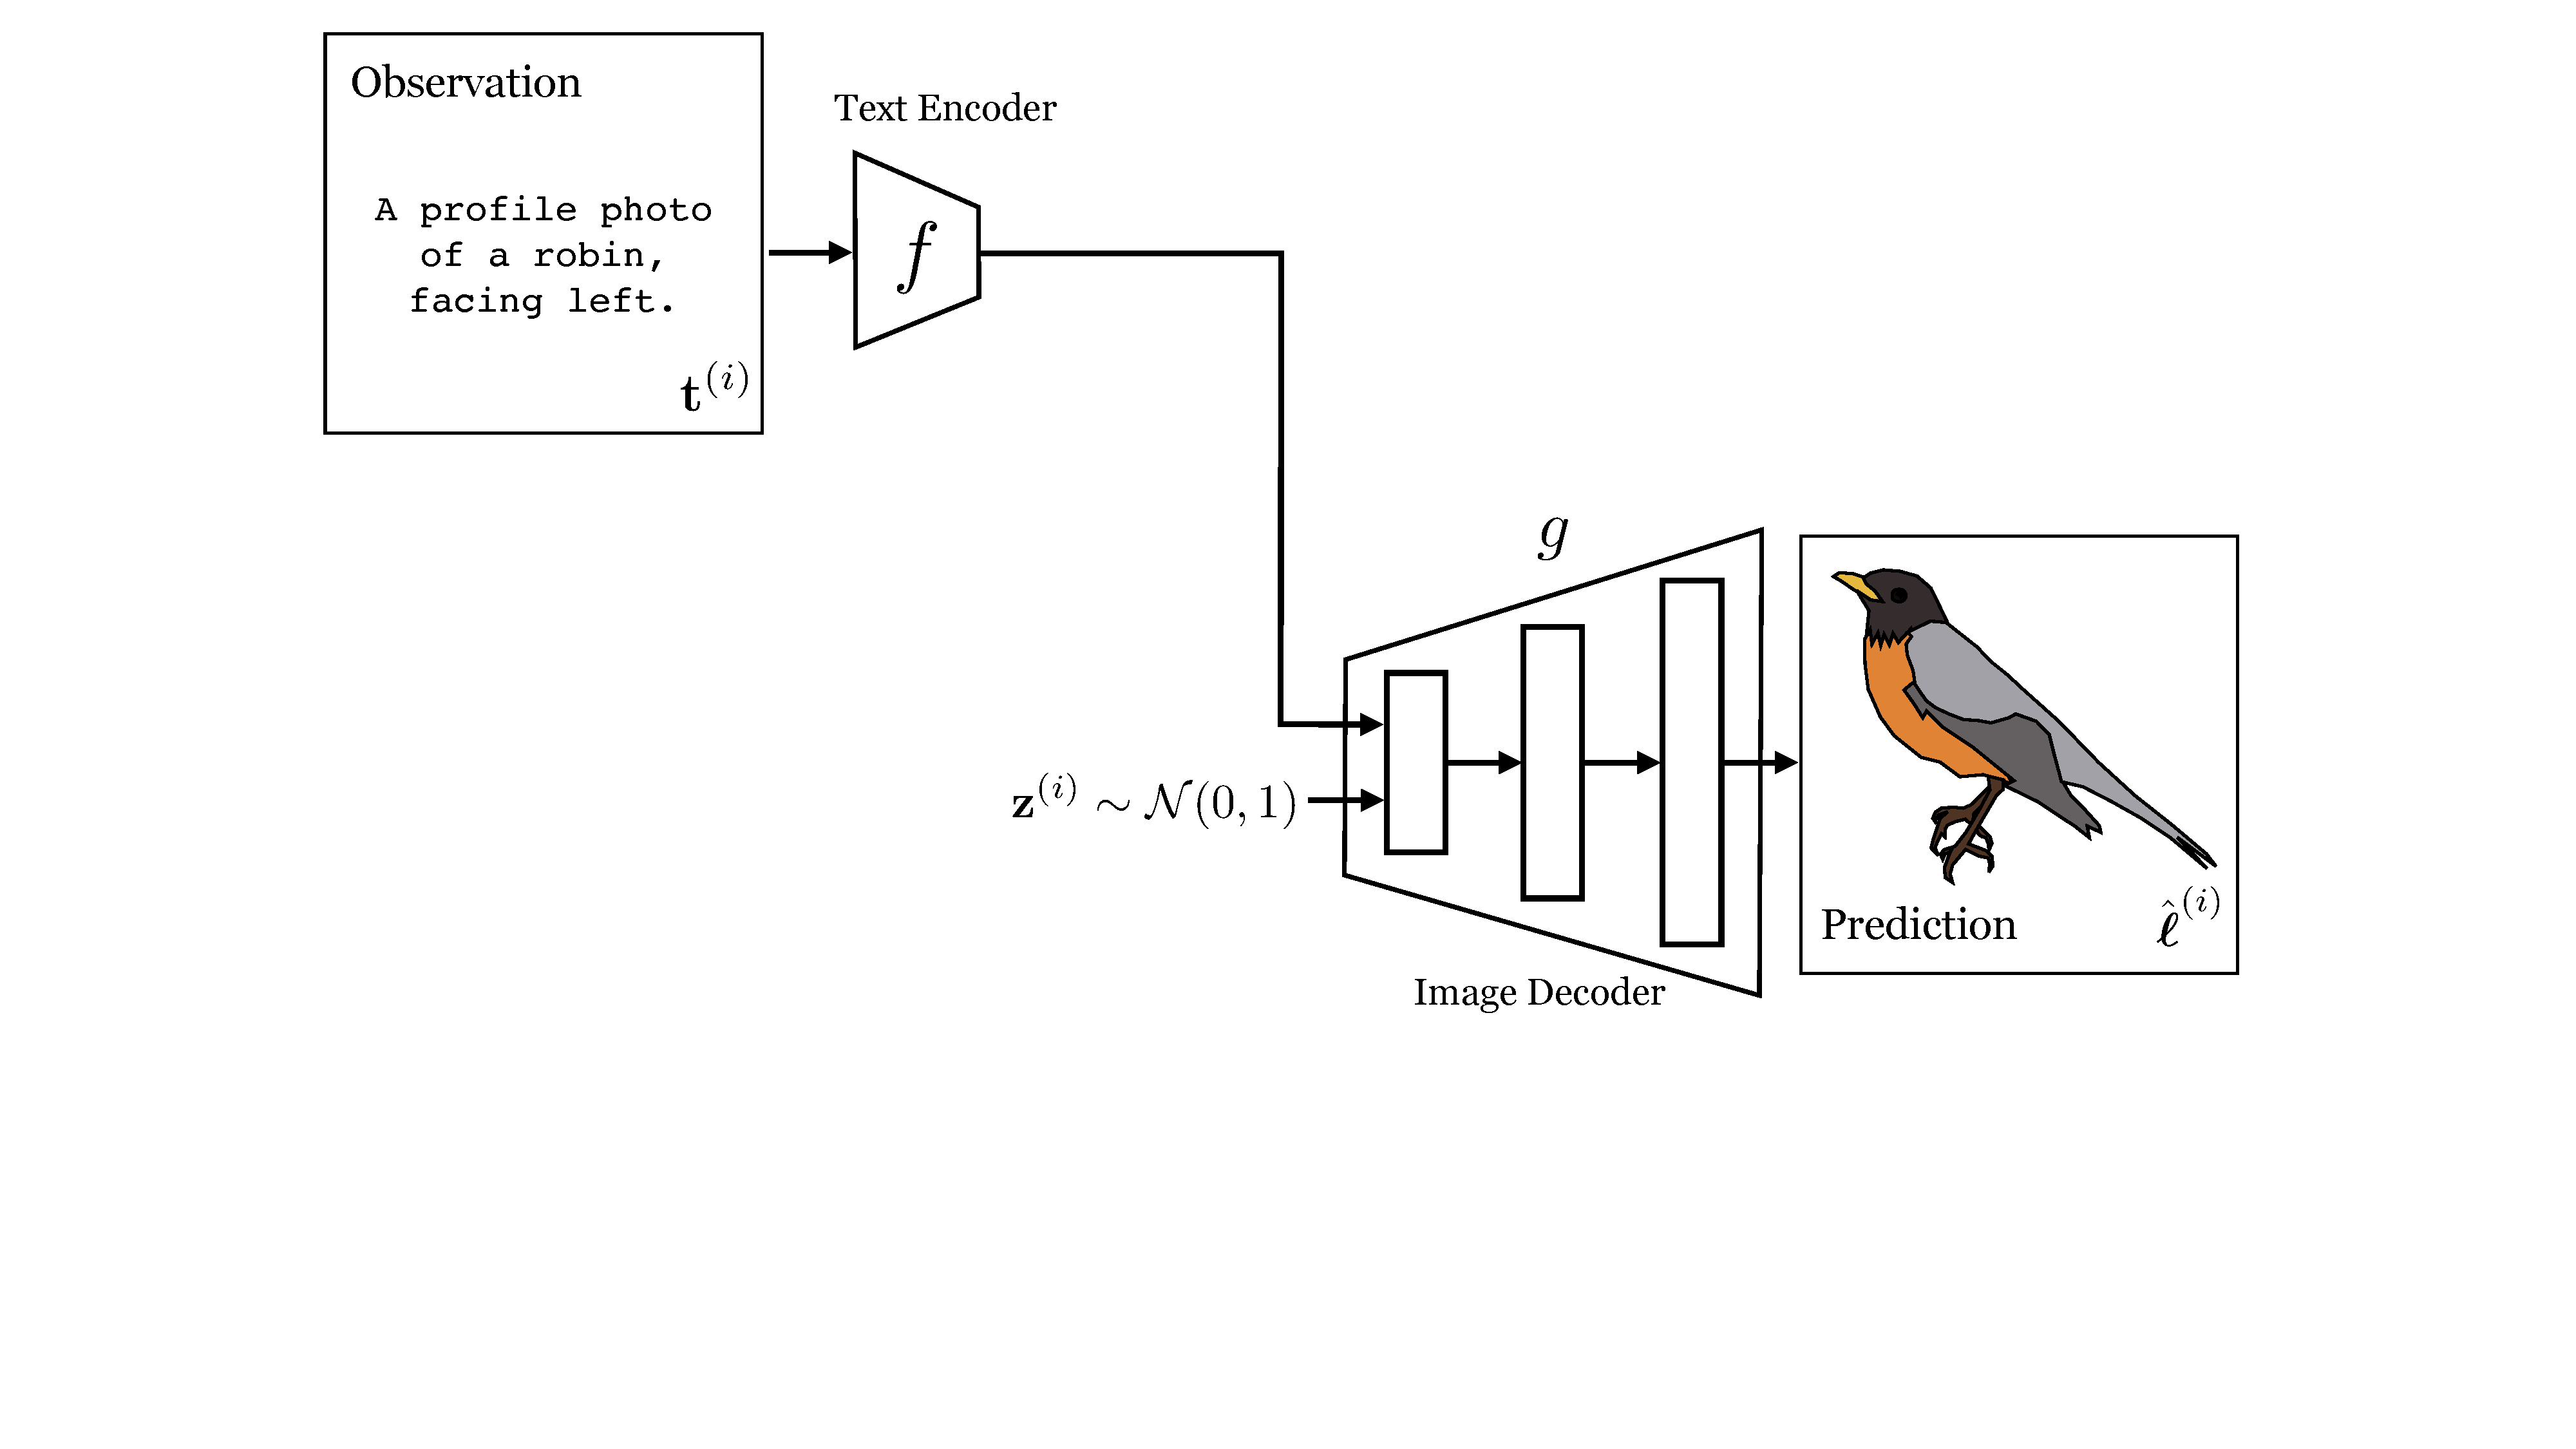
\includegraphics[width=1.0\linewidth]{./figures/vision_and_language/text2im_VAE_sampling.pdf}
    }
    \caption{Sampling from a trained cVAE.}
    \label{fig:vision_and_language:text2im_VAE_sampling}
\end{figure}
\begin{figure}[h!]
    \centerline{
        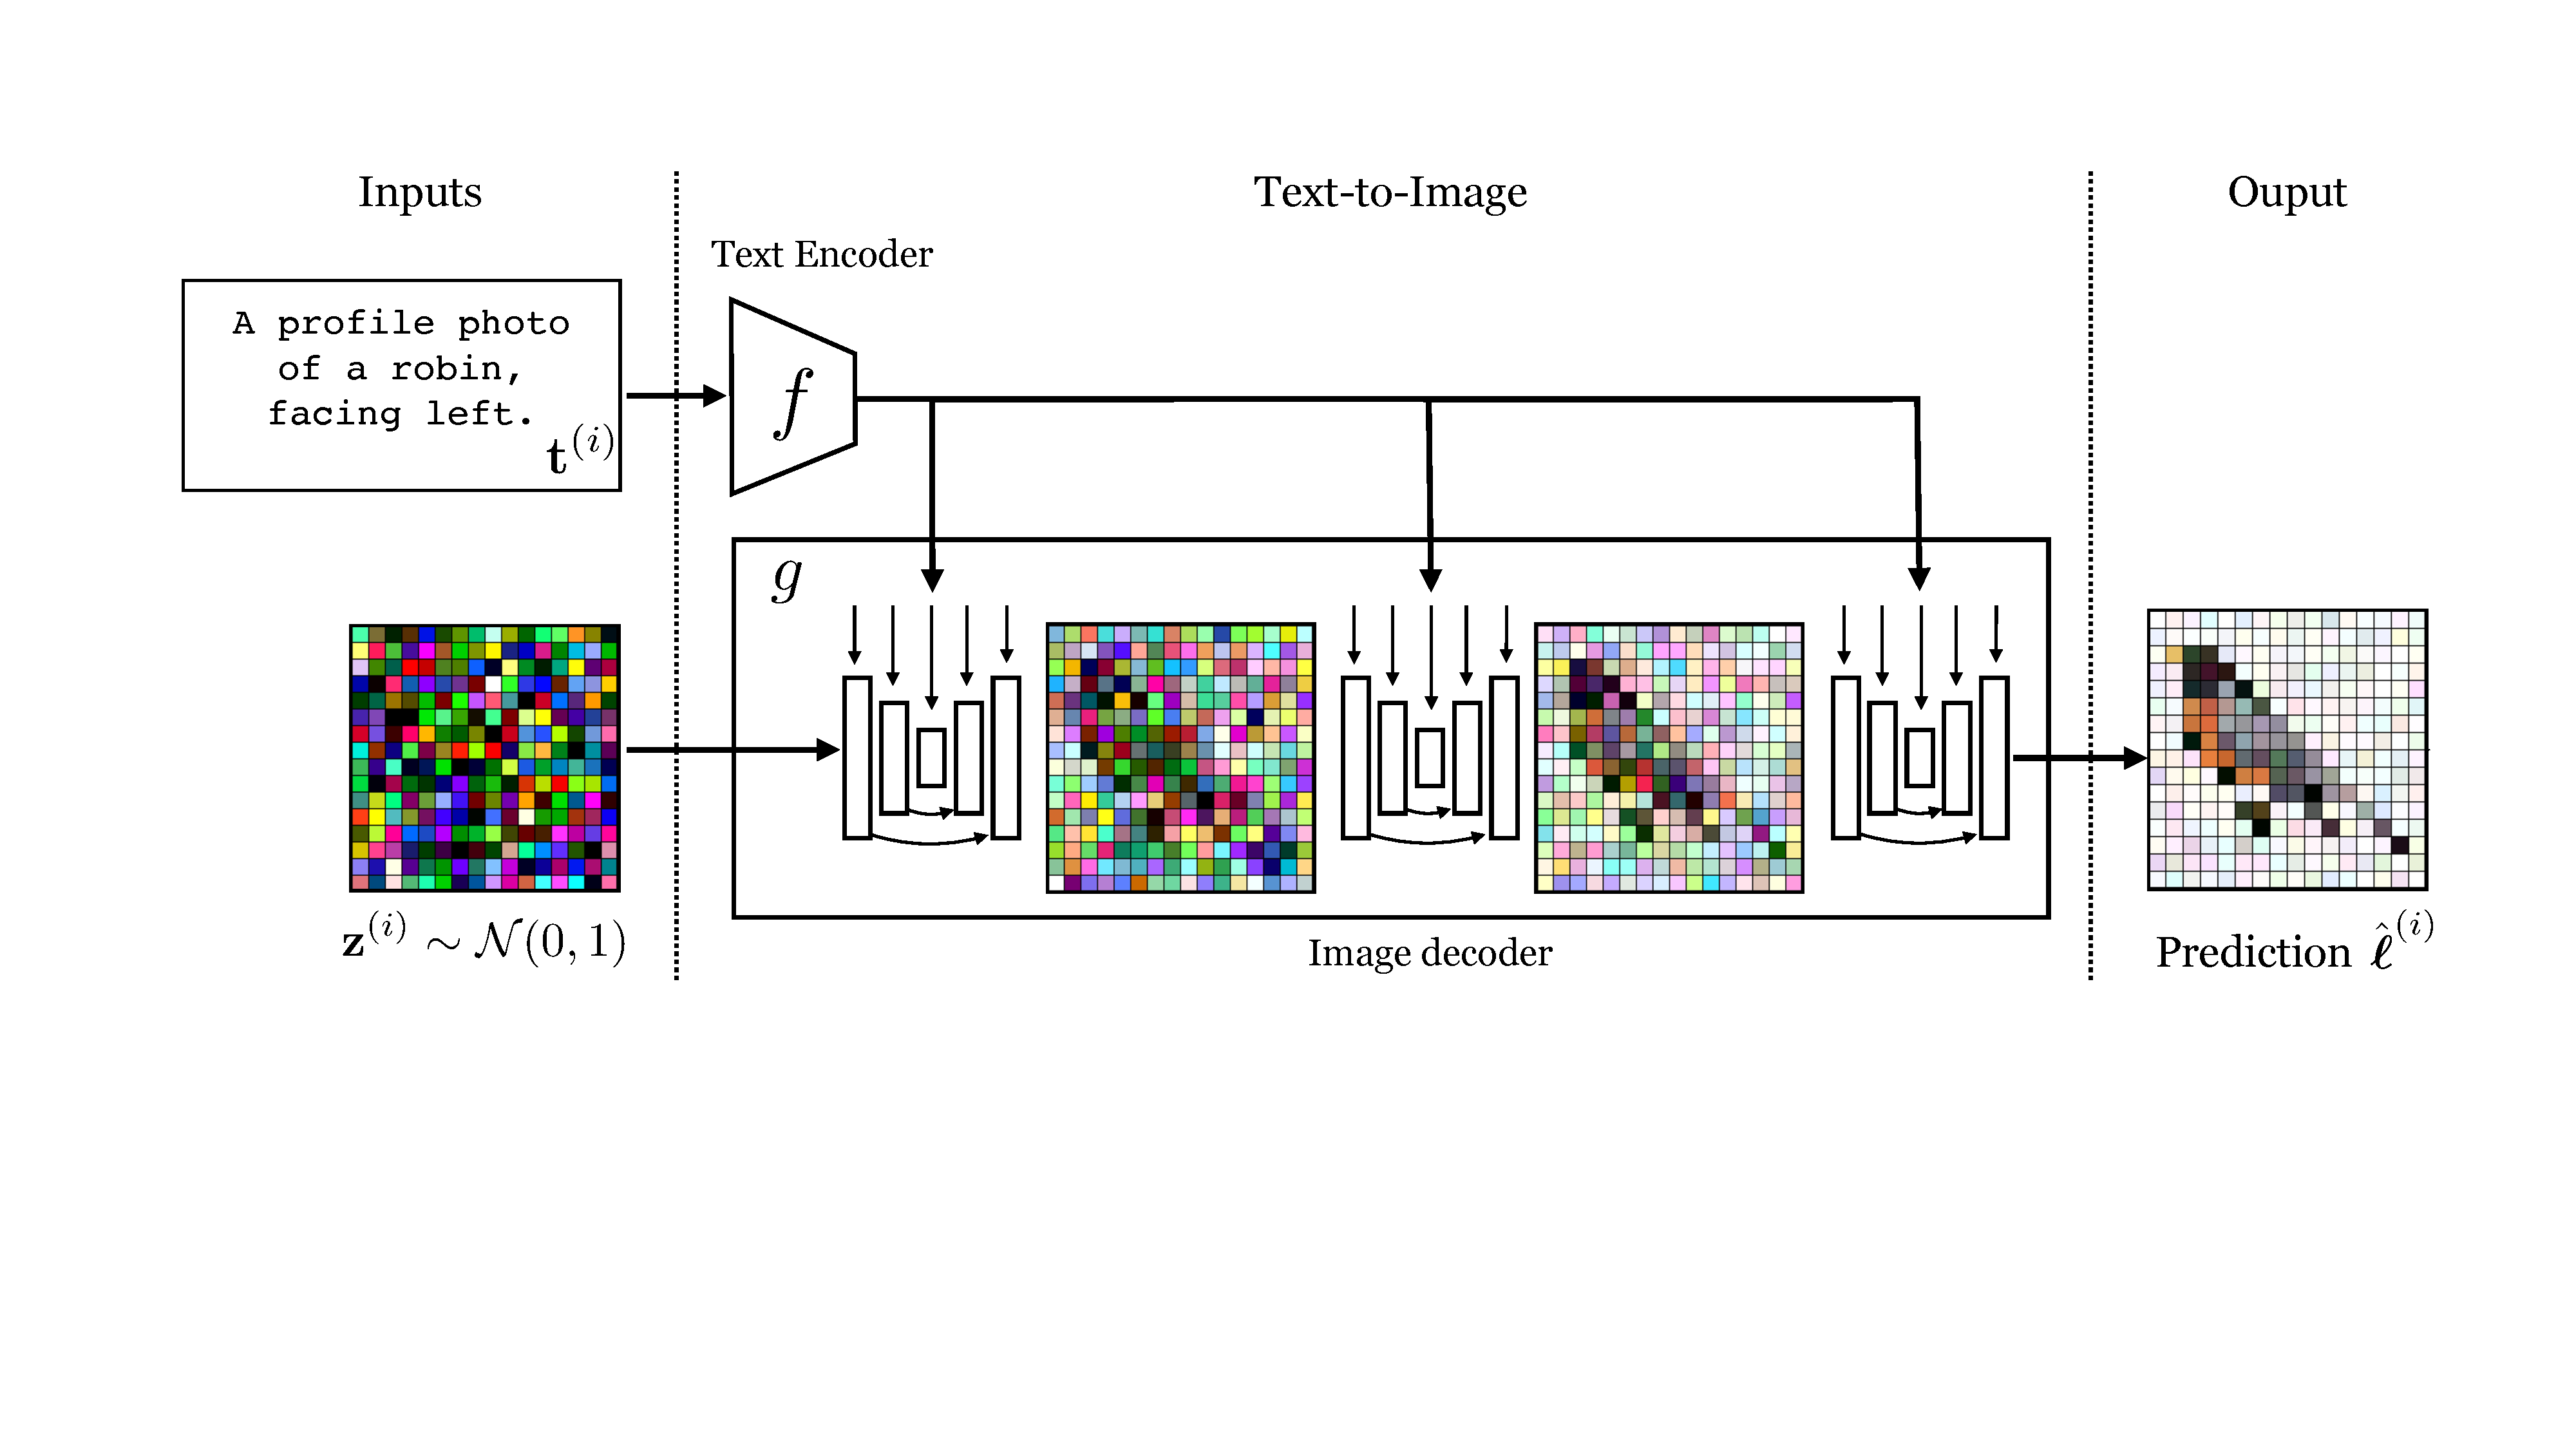
\includegraphics[width=1.0\linewidth]{./figures/vision_and_language/text2im_diffusion_model.pdf}
    }
    \caption{A text-to-image diffusion model.}
    \label{fig:vision_and_language:text2im_diffusion_model}
\end{figure}
Notice that \fig{\ref{fig:vision_and_language:text2im_diffusion_model}} is actually very similar to \fig{\ref{fig:vision_and_language:text2im_VAE_sampling}}. A conditional diffusion model is in fact very similar to a cVAE. At sampling time, both take as input text and Gaussian noise. The VAE uses a network that directly maps these inputs to an image, in a single forward pass. The diffusion model, in contrast, maps to an image via a chain of denoising steps, each of which is a forward pass through a neural network. See \cite{NEURIPS2021_b578f2a5} for a discussion of the connection between diffusion models and VAEs.


\subsection{Image-to-Text}\label{sec:VLMs:im2text}
Naturally, we can also translate in the opposite direction. We just need to use an \textit{image encoder} (rather than a text encoder) and a \textit{text decoder} (rather than a text encoder). In this direction, the problem can be called \index{Image-to-text}\textbf{image-to-text} or \index{Image captioning}\textbf{image captioning}. This kind of translation is very useful because text is a ubiquitous and general-purpose interface between almost all domains of human knowledge (we use language to describe pretty everything we do and everything we know). So, if we can translate images to text then we link imagery to many other domains of knowledge.

As an example of an image-to-text system, we will use a transformer to map the input image to a set of tokens, and we will then feed these tokens as input to an autoregressive text decoder, which is also implemented with a transformer. See \cite{li2023blip2} for an example of a system that uses this general approach. \Fig{\ref{fig:VLMs:im2text}} shows this architecture.
\begin{figure}[h]
    \centerline{
        \begin{tikzpicture}
            %
            %% Image encoder
            \def\Nnodes{3}
            \def\Nnodesplusone{4}
            \def\Nlayers{3}
            \def\layerheight{1.2}
            \def\neuronrad{0.3}
            \def\neuronstep{0.7}
            \begin{scope}[shift={(\neuronstep*-3, \layerheight*-2)}]
                % image patches
                \draw (\neuronstep,-\layerheight) node[inner sep=0] {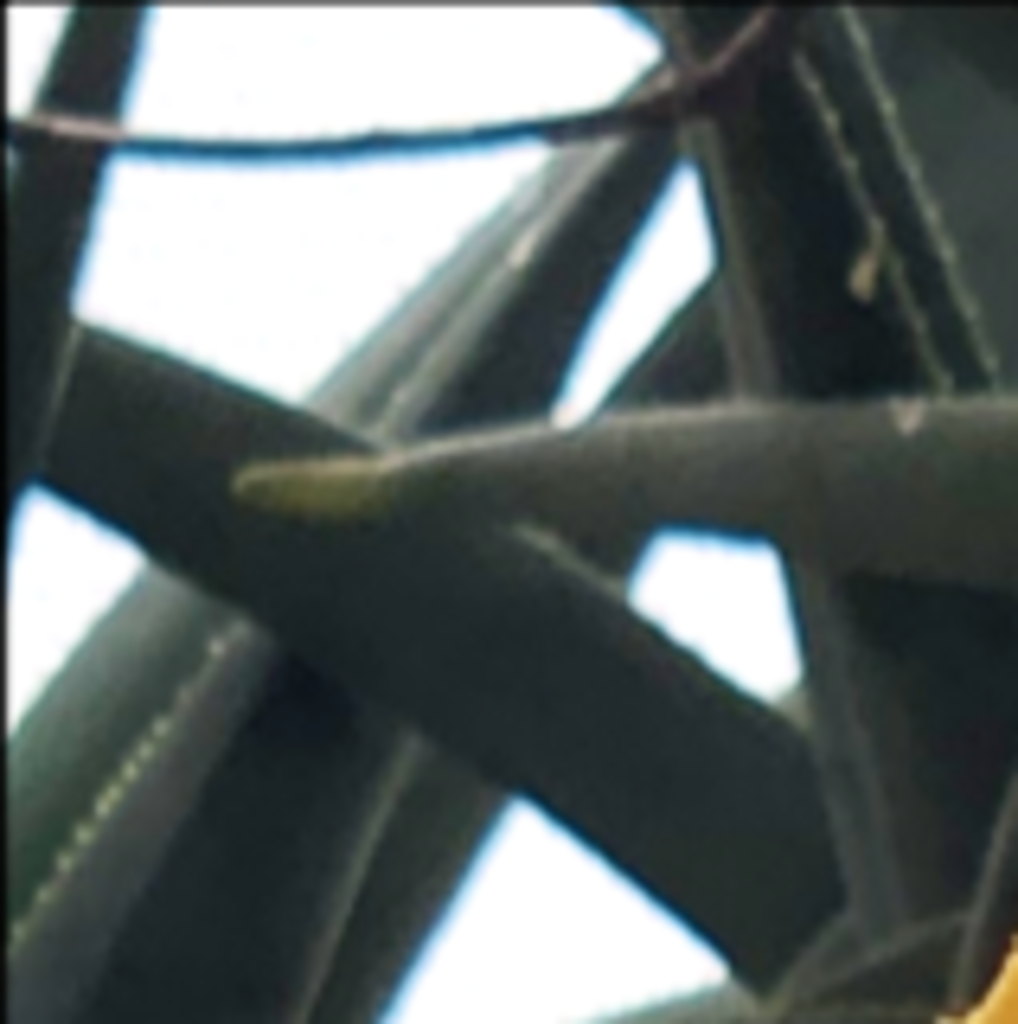
\includegraphics[width=0.05\linewidth]{./figures/vision_and_language/yellow_bird_patches/patch_0_0.png}};
                \draw (\neuronstep*2,-\layerheight) node[inner sep=0] {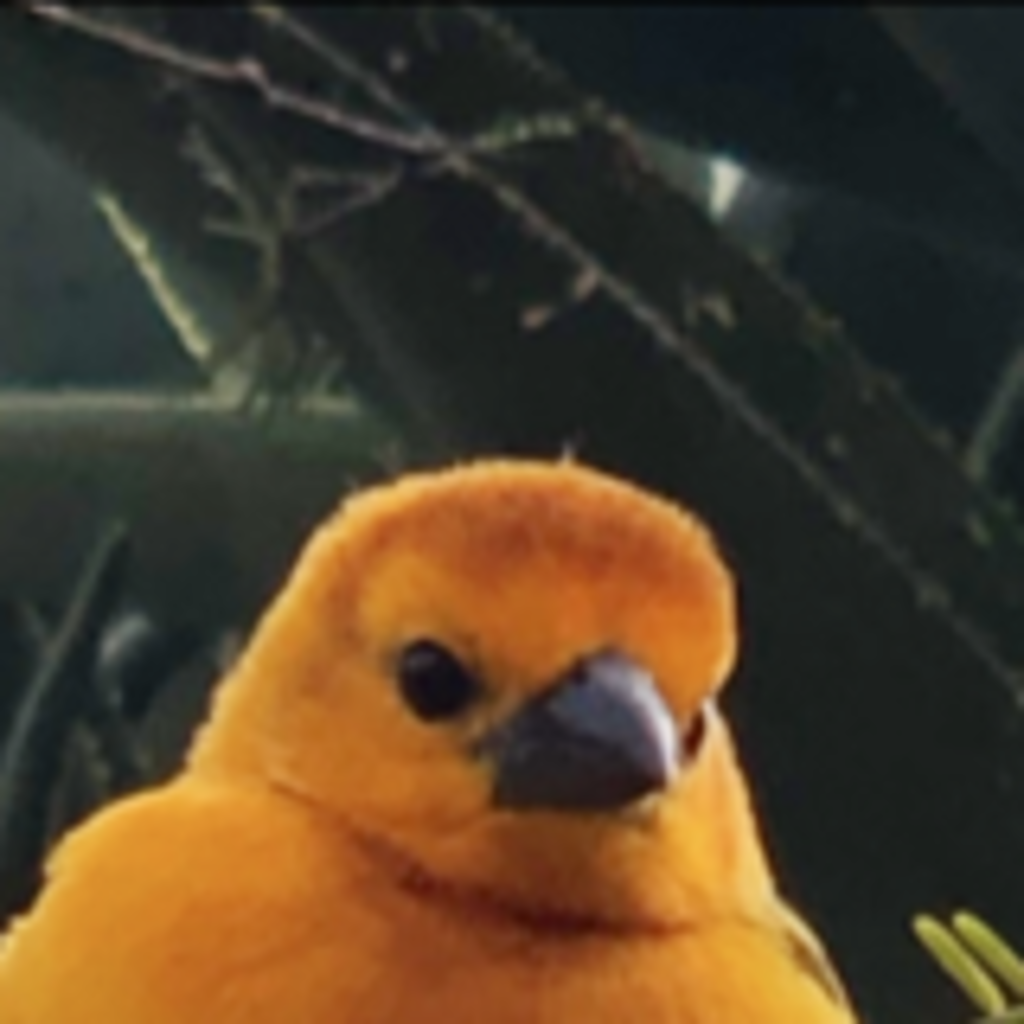
\includegraphics[width=0.05\linewidth]{./figures/vision_and_language/yellow_bird_patches/patch_1_0.png}};
                \draw (\neuronstep*3,-\layerheight) node[inner sep=0] {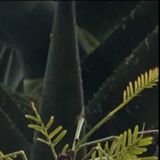
\includegraphics[width=0.05\linewidth]{./figures/vision_and_language/yellow_bird_patches/patch_2_0.png}};
                % token projection layer
                \foreach \x in {1,...,\Nnodes} {
                        \draw [thick] [nn_edge] (\neuronstep*\x,\neuronrad-\layerheight) -- (\neuronstep*\x,\layerheight-\neuronrad-\layerheight);
                    }
                % image tokens first layer
                \foreach \x in {1,...,\Nnodes} {
                        \foreach \y in {1,...,\Nlayers} {
                                \draw (\neuronstep*\x-\neuronrad/4,\layerheight*\y-\layerheight-\neuronrad) rectangle ++(\neuronrad/2,\neuronrad*2);
                            }
                    }
                % mixing layer 1
                \foreach \xi in {1,...,\Nnodes} {
                        \foreach \xj in {1,...,\Nnodes} {
                                \draw [thick] [nn_edge] (\neuronstep*\xi,\neuronrad) -- (\neuronstep*\xj,\layerheight-\neuronrad);
                            }
                    }
                % pointwise nonlinearity 1
                \foreach \x in {1,...,\Nnodes} {
                        \draw [thick] [nn_edge] (\neuronstep*\x,\layerheight+\neuronrad) -- (\neuronstep*\x,\layerheight*2-\neuronrad);
                    }
                % cross-attention
                \foreach \xi in {1,...,\Nnodes} {
                        \foreach \xj in {1,...,\Nnodes} {
                                \draw [thick, color=cross_attn_color] [nn_edge] (\neuronstep*\xi,\layerheight*2+\neuronrad) -- (\neuronstep*\xj+\neuronstep*4,\layerheight*3.5-\neuronrad);
                            }
                    }
                %
                \draw [thick] [nn_edge] (0.2,0) arc
                    [
                        start angle=250,
                        end angle=90,
                        x radius=0.4cm,
                        y radius =0.3cm
                    ] ;
                \draw (0.3, 0) node {$\Big\{$};
                \draw (-1.1,0.3) node {$\texttt{self-attn}$};
                %
                \draw [thick, color=cross_attn_color] [nn_edge] (0.2,\layerheight*2) arc
                    [
                        start angle=250,
                        end angle=90,
                        x radius=0.4cm,
                        y radius =0.4cm
                    ] ;
                \draw (0.3, \layerheight*2) node {$\Big\{$};
                \draw (-1.2,\layerheight*2+0.4) node {$\texttt{cross-attn}$};
            \end{scope}
            %
            %% Text decoder
            %
            \def\Nnodes{3}
            \def\Nnodesplusone{4}
            \def\Nlayers{4}
            \def\layerheight{1.2}
            \def\neuronrad{0.3}
            \def\neuronstep{0.7}
            % time bars
            \foreach \x in {1,...,\Nnodesplusone} {
                    \draw [dotted, thick] (\neuronstep*\x,-\layerheight*0.25) -- (\neuronstep*\x,\layerheight*3.75);
                }
            % text inputs
            \node [rotate=45] at (\neuronstep,-\layerheight) {\small \texttt{A}};
            \node [rotate=45] at (\neuronstep*2,-\layerheight) {\small \texttt{yellow}};
            \node [rotate=45] at (\neuronstep*3,-\layerheight) {\small \texttt{bird}};
            % token input projection layer
            \foreach \x in {1,...,\Nnodes} {
                    \draw [thick] [nn_edge] (\neuronstep*\x,\neuronrad-\layerheight) -- (\neuronstep*\x,\layerheight-\neuronrad-\layerheight);
                }
            % token output projection layer
            \foreach \x in {2,...,\Nnodesplusone} {
                    \draw [thick] [nn_edge] (\neuronstep*\x,\neuronrad+\layerheight*3.5) -- (\neuronstep*\x,\layerheight-\neuronrad+\layerheight*3.5);
                }
            % text outputs
            \node [rotate=45] at (\neuronstep*2,\layerheight*4.5) {\small \texttt{yellow}};
            \node [rotate=45] at (\neuronstep*3,\layerheight*4.5) {\small \texttt{bird}};
            \node [rotate=45] at (\neuronstep*4,\layerheight*4.5) {\small \texttt{sitting}};

            % text tokens on first layer
            \foreach \x in {1,...,\Nnodes} {
                    \draw [fill=white] (\neuronstep*\x-\neuronrad/4,\layerheight-\layerheight-\neuronrad) rectangle ++(\neuronrad/2,\neuronrad*2);
                }
            % mixing layer 1
            \foreach \xi in {1,...,\Nnodes} {
                    \foreach \xj in {1,...,\Nnodes} {
                            \pgfmathsetmacro\ximinusone{\xi-1}
                            \ifthenelse{\xj>\ximinusone}{
                                \draw [thick] [nn_edge] ($(\neuronstep*\xi,\neuronrad)$) -- ($(\neuronstep*\xj+\neuronstep,1.5*\layerheight-\neuronrad)$);
                            }{}
                        }
                }
            \begin{scope}[shift={(0,\layerheight*0.5)}]
                % text tokens on subsequent layers
                \foreach \x in {1,...,\Nnodes} {
                        \foreach \y in {2,...,\Nlayers} {
                                \draw [fill=white] (\neuronstep*\x+\neuronstep-\neuronrad/4,\layerheight*\y-\layerheight-\neuronrad) rectangle ++(\neuronrad/2,\neuronrad*2);
                            }
                    }
                % pointwise nonlinearity
                \foreach \x in {1,...,\Nnodes} {
                        \draw [thick] [nn_edge] (\neuronstep*\x+\neuronstep,\layerheight+\neuronrad) -- (\neuronstep*\x+\neuronstep,\layerheight*2-\neuronrad);
                    }
                % mixing layer 2
                \foreach \xi in {1,...,\Nnodes} {
                        \foreach \xj in {1,...,\Nnodes} {
                                \pgfmathsetmacro\ximinusone{\xi-1}
                                \ifthenelse{\xj>\ximinusone}{
                                    \draw [thick] [nn_edge] ($(\neuronstep*\xi+\neuronstep,\layerheight*2+\neuronrad)$) -- ($(\neuronstep*\xj+\neuronstep,\layerheight*3-\neuronrad)$);
                                }{}
                            }
                    }
            \end{scope}
            \draw [thick] [nn_edge] (2.5+\neuronstep,0) arc
                [
                    start angle=-70,
                    end angle=90,
                    x radius=0.4cm,
                    y radius =0.4cm
                ] ;
            \draw (2.4+\neuronstep, 0) node {$\Big\}$};
            \draw (3.5+\neuronstep,0.6*\layerheight) node {$\texttt{causal}$};
            \draw (3.8+\neuronstep,0.3*\layerheight) node {$\texttt{self-attn}$};
            %
            \draw [thick] [nn_edge] (2.5+\neuronstep,\layerheight*2.5) arc
                [
                    start angle=-70,
                    end angle=90,
                    x radius=0.4cm,
                    y radius =0.3cm
                ] ;
            \draw (2.4+\neuronstep, \layerheight*2.5) node {$\Big\}$};
            \draw (3.5+\neuronstep,0.4*\layerheight+\layerheight*2.5) node {$\texttt{causal}$};
            \draw (3.8+\neuronstep,0.1*\layerheight+\layerheight*2.5) node {$\texttt{self-attn}$};
            %
            \draw (-\neuronstep*7,-\layerheight*3.25) -- (-\neuronstep*7,\layerheight*0.25);
            \node [fill=white, rotate=90] at (-\neuronstep*7, -\layerheight*1.5) {Image Encoder};
            \draw (\neuronstep*8.5,-\layerheight*0.25) -- (\neuronstep*8.5,\layerheight*4.75);
            \node [fill=white, rotate=90] at (\neuronstep*8.5, \layerheight*2.5) {Text Decoder};
        \end{tikzpicture}
    }
    \caption{Image-to-text using a small transformer with cross-attention. The edges in gray are cross-attention edges. Many variations of this architecture are possible. For example, each layer of the text encoder could cross-attend to the output image tokens. Or, the image encoder could compress all its input tokens into a single output token that represents the entire photo; this output token would then get cross-attended by the text decoder. This approach could save memory and computation time.}
    \label{fig:VLMs:im2text}
\end{figure}

There is one special layer to point out, the \index{Attention!Cross-attention}\textbf{cross-attention} layer (\texttt{cross-attn}). This layer addresses the question of how to insert image tokens into a text model. The answer is quite simple: just let the text tokens attend to the image tokens. The image tokens will emit their value vectors which will be mixed with the text token value vectors according to the attention weights to produce the next layer of tokens in the text decoder.

Here are the equations for a cross-attention layer:
\begin{align}
    \mathbf{Q}_{t} = \mathbf{T}_{t}\mathbf{W}_{t,q}^\transpose                                                  \\
    \mathbf{K}_{\img} = \mathbf{T}_{\img}\mathbf{W}_{\img,k}^\transpose                                         \\
    \mathbf{V}_{\img} = \mathbf{T}_{\img}\mathbf{W}_{\img,v}^\transpose                                         \\
    \mathbf{A}_{\texttt{cross}} = \texttt{softmax}(\frac{\mathbf{Q}_{t}\mathbf{K}_{\img}^\transpose}{\sqrt{m}}) \\
    \mathbf{T}_{\texttt{out}, \texttt{cross}} = \mathbf{A}_{\texttt{cross}}\mathbf{V}_{\img}
\end{align}
where variables subscripted with $t$ are associated with text tokens and variables subscripted with $\img$ are associated with image tokens.

Then, the tokens output by cross-attention can be combined with tokens output by self-attention by weighted summation:
\begin{align}
    \mathbf{T} = w_{\texttt{cross}}\mathbf{T}_{\texttt{out}, \texttt{cross}}  + w_{\texttt{self}}\mathbf{T}_{\texttt{out}, \texttt{self}}
\end{align}
where $\mathbf{T}_{\texttt{out}, \texttt{self}}$ is regular self-attention on the input text token $\mathbf{T}_t$, and $w_{\texttt{cross}}$ and $w_{\texttt{self}}$ are optional learnable weights.

The text decoder is an autoregressive model (\sect{\ref{sec:generative_models:autoregressive}}) that uses causal attention (\sect{\ref{sec:transformers:masked_attention}}) to predict the next word in the sentence given the previous words generated so far. In this strategy, the input to the text decoder is the tokens representing the previous words in the training data caption that describes the image. At sampling time, the model is run sequentially, where for each next word generated it autoregressively repeats, with that word being added to the input sequence of tokens. The text tokens themselves are produced by tokenizing the input words, for example, via byte-pair encodings or word-level encodings (the latter is shown in the figure).

\section{Text as a Visual Representation}

One way of thinking about image-to-text is as yet another visual encoder, where text is the visual representation. Just like we can represent an image in terms of its frequencies (Fourier transform), its semantics and geometry (scene understanding), or its feature embeddings (DINO~\cite{caron2021emerging}, CLIP~\cite{radford2021learning}, and others), we can also represent it in terms of a textual description of its content.

% We have seen many kinds of visual representations in this book. In this section, we will consider text as another kind of visual representation.

% What do LLMs know about vision. GPT-4 tikz, ViperGPT, etc.

In \fig{\ref{fig:vision_and_language:different_visual_representations}} we show an image represented in several ways (the depth map is produced by MiDaS~\cite{Ranftl2022} and the text is produced by BLIP2~\cite{li2023blip2}):
\begin{figure}[h!]
    \centerline{
        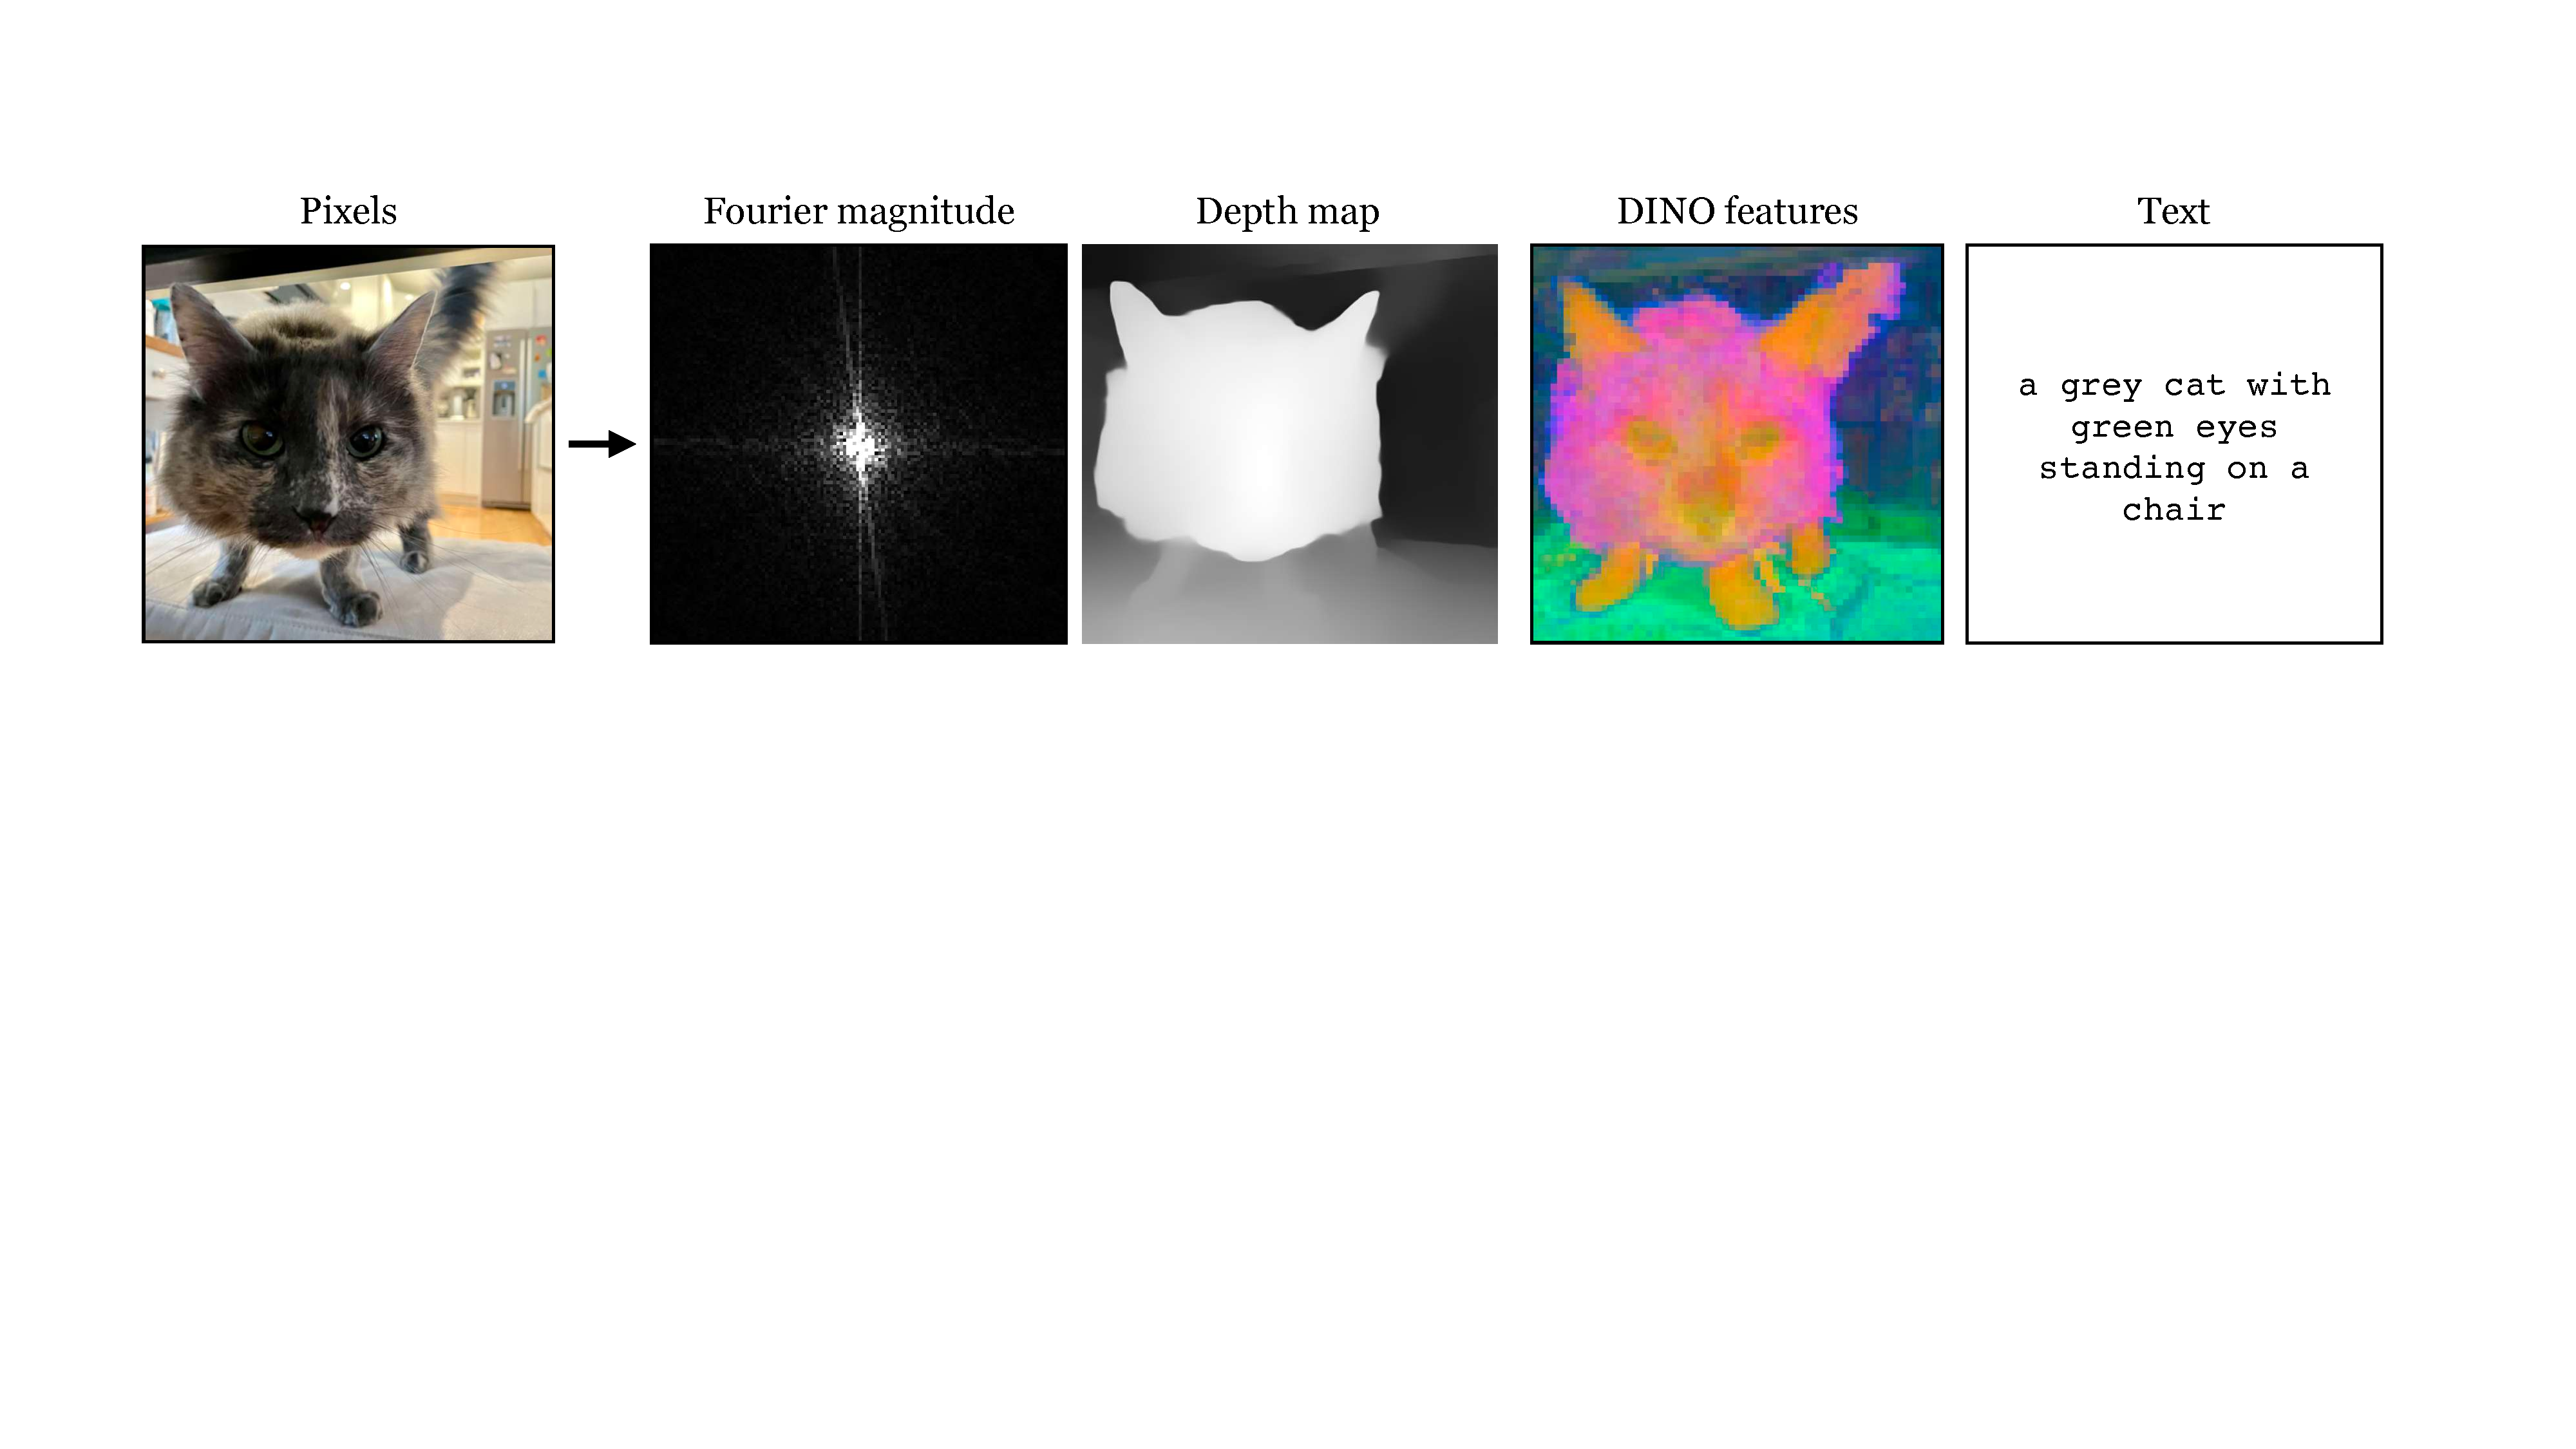
\includegraphics[width=1.0\linewidth]{figures/vision_and_language/different_visual_representations.pdf}
    }
    \caption{Four representations computed from the input on the left. The input image itself (its pixel values) is in fact a fifth representation of the scene.}
    \label{fig:vision_and_language:different_visual_representations}
\end{figure}

%\marginnote{The depth map is produced by MiDaS~\cite{Ranftl2022} and the text is produced by BLIP2~\cite{li2023blip2}.}[-0.6cm]

Think about the relative merits of each of these representations, and what advantages or disadvantages text might have over these other kinds of visual representation.

Text is a powerful visual representation because it interfaces with language models. This means that after translating an image into text we can use language models to reason about the image contents.


\section{Visual Question Answering}

As AI systems become more general purpose, one goal is to make a vision algorithm that is fully general, so that you can ask it any question about an image. This is akin to a Turing test~\cite{turing2009computing} for visual intelligence. \index{Visual question answering}\textbf{Visual question answering} (\textbf{VQA}) is one formulation of this goal~\cite{antol2015vqa}. The problem statement in VQA is to make a system that maps an image and a textual question to a textual answer, as shown in \fig{\ref{fig:vision_and_language:VQA_examples}}.
\begin{figure}
    \centerline{
        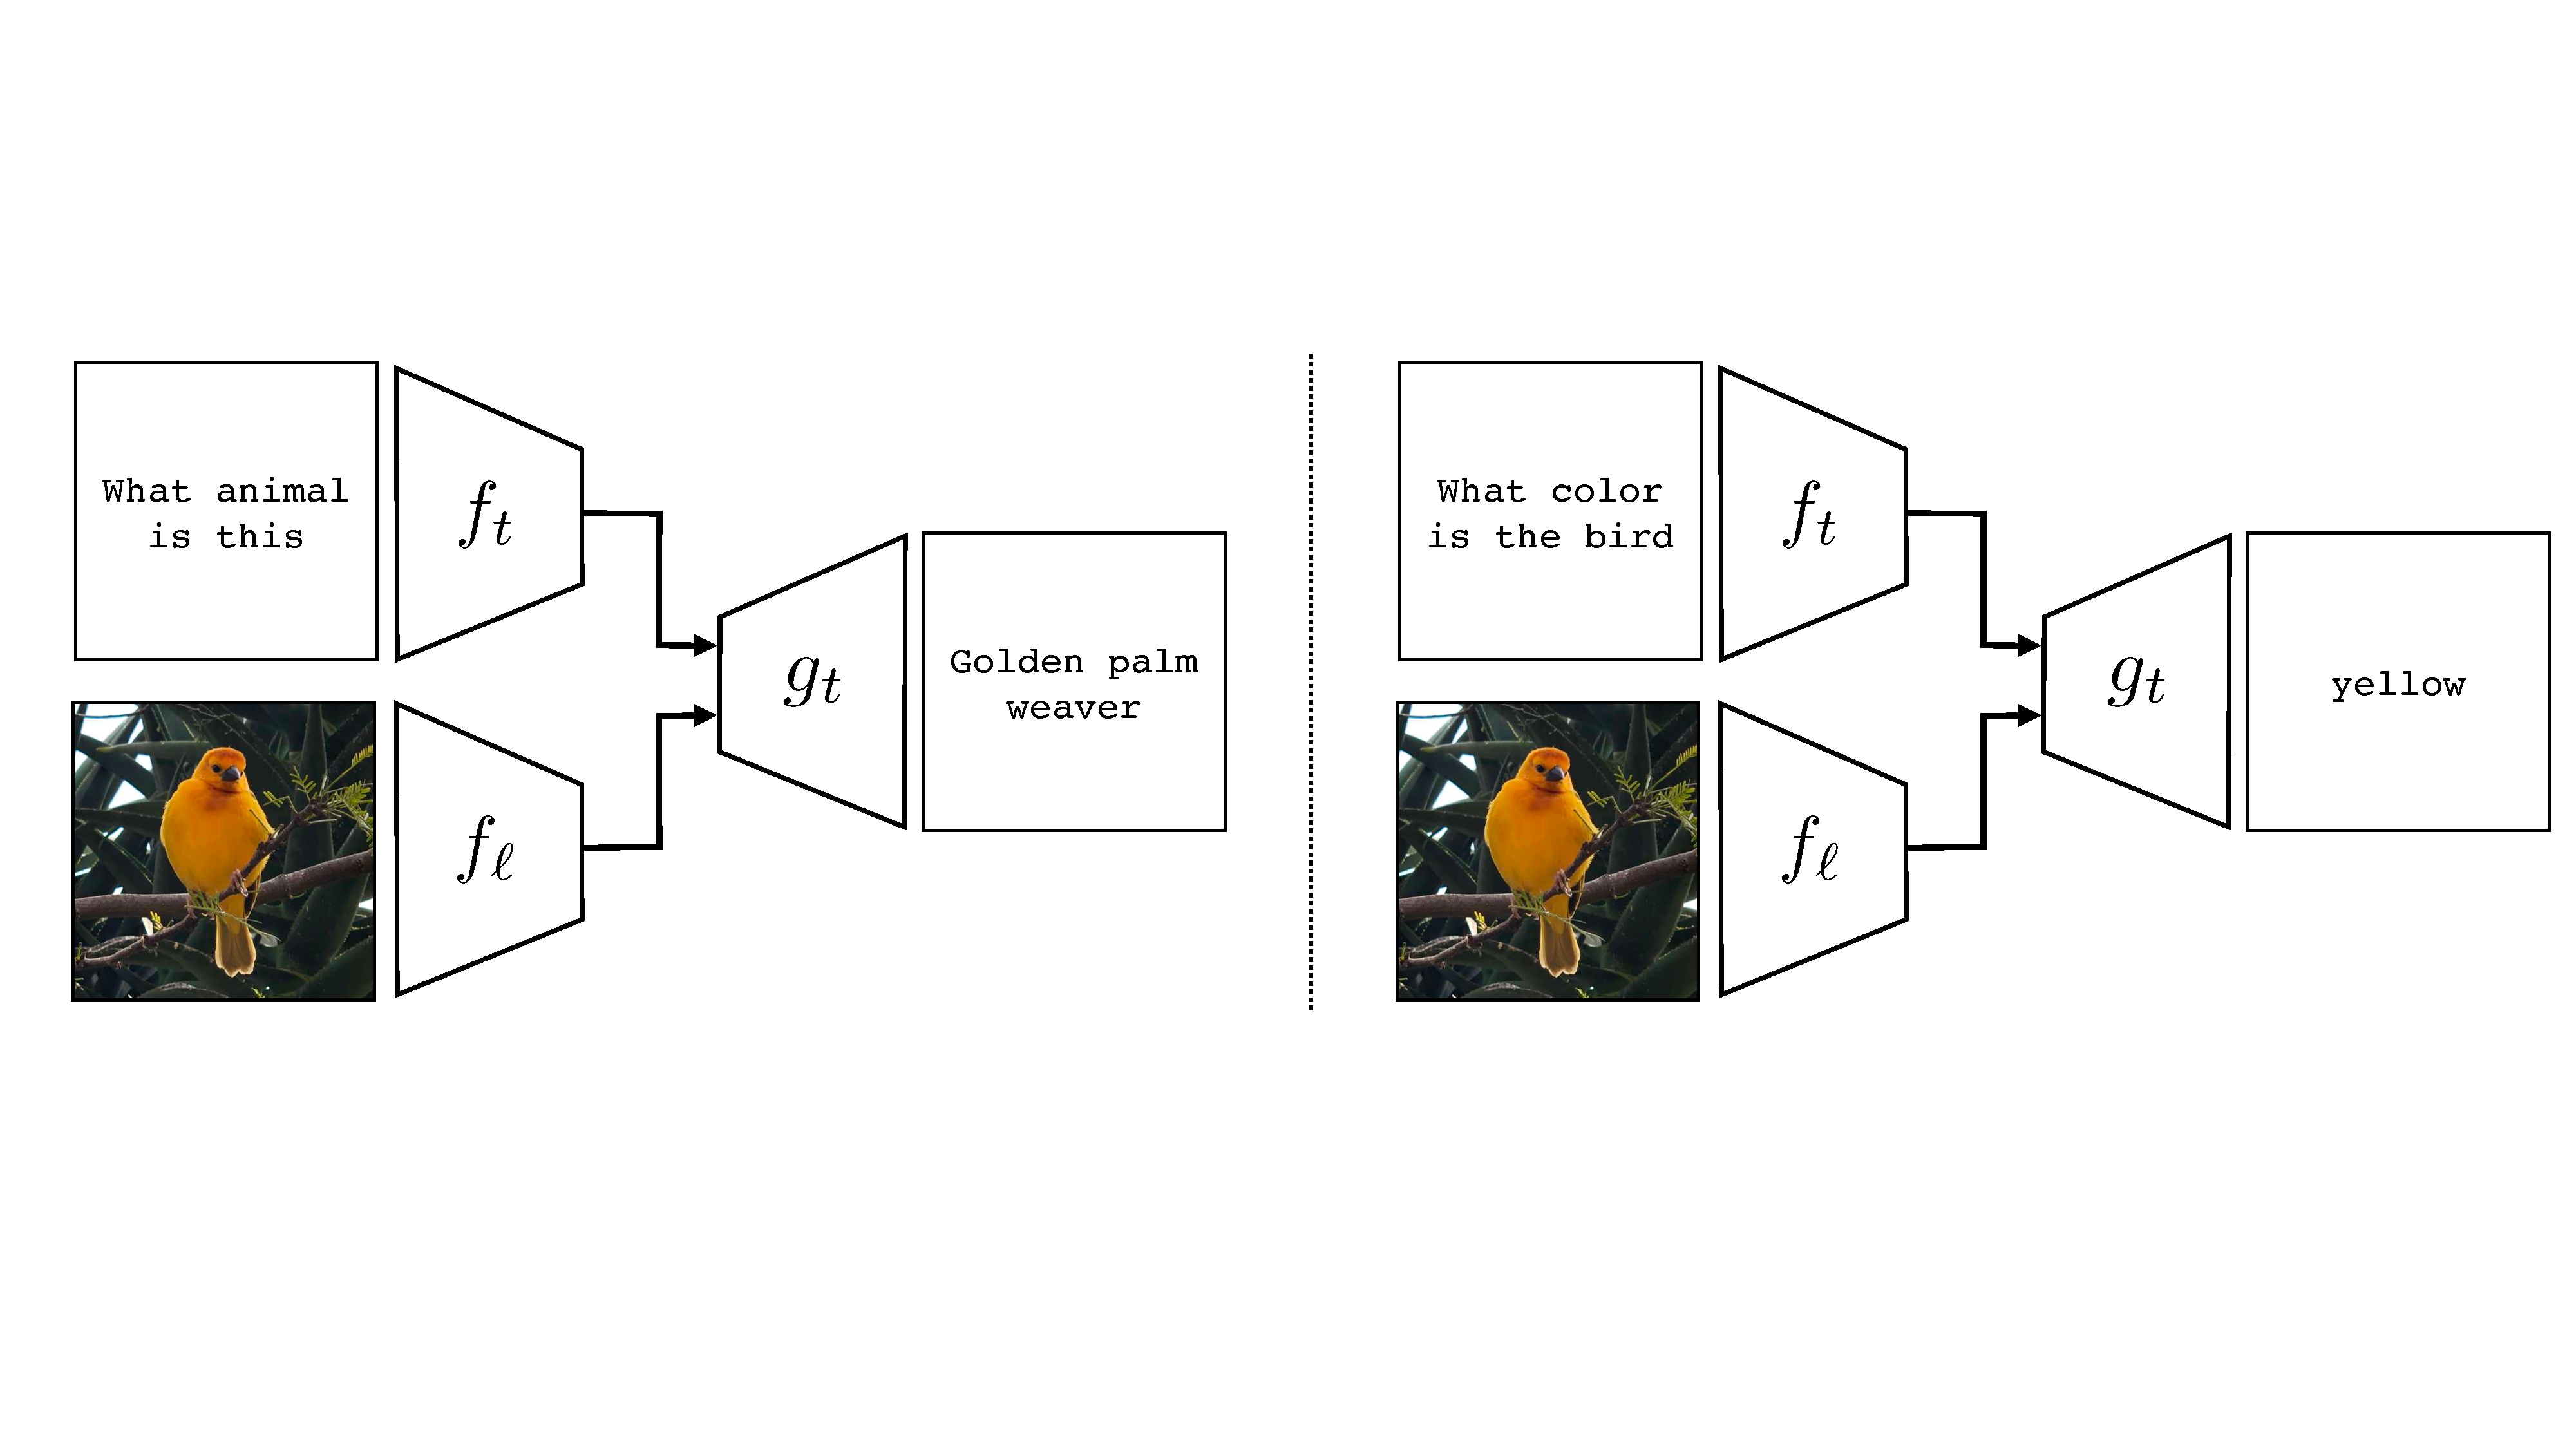
\includegraphics[width=1.0\linewidth]{figures/vision_and_language/VQA_examples.pdf}
    }
    \caption{An example VQA system.}
    \label{fig:vision_and_language:VQA_examples}
\end{figure}

\marginnote{By now you have seen several ways to build image and text encoders as well as decoders, and how to put them together. As an exercise, think about how you might implement the VQA system shown here, using the tools from elsewhere in this chapter and book. See if you can modify the transformer architecture in \fig{\ref{fig:VLMs:im2text}} to solve this problem.}[-2cm]

In this chapter, we have already seen all the tools necessary to create a VQA system; you just need a text encoder (for the question), an image encoder (for the image you are asking the question about), and a text decoder (for the answer). These can be hooked together using the same kinds of tools we have seen earlier in this chapter. The critical piece is just to acquire training data of VQA examples, each of which takes the form of a tuple \{[\texttt{question}, \texttt{image}], \texttt{answer}\}. For a representative example of how to implement a VQA model using transformers, see \cite{li2023blip2}.

%These language models can also interface with other systems that have language-based interfaces. For example, a language model can write Python code, based on the image contents, and then execute that code, calling Python libraries that do further analysis on the image. This can be a powerful way to approach visual question answering, which we will see in \sect{\ref{sec:VLMs:VQA}}. Examples of this approach are \cite{visprog}, \cite{vipergpt}, and \cite{visualchatgpt}.

%Visual Turing test, being able to answer question, 20 questions, Geman and Geman.

%Visual routines. Modular nets (Jacob Andreas).


%\section{Symbolic vs non-symbolic visual representations}



\section{Concluding Remarks}

From the perspective of vision, language is a perceptual representation. It is a way of describing ``what is where''\footnote{``To know what is where by looking'' is how David Marr defined the vision in his seminal book on the subject~\cite{Marr82}.} and much more in a low-dimensional and abstracted format that interfaces well with other domains of human knowledge. There are many theories of how human language evolved, and what it is useful for: communication, reasoning, abstract thought. In this chapter, we have suggested another: language is, perhaps, the result of perceptual representation learning over the course of human evolution and cultural development. It's one of the main formats brains have arrived at as the best way to represent the ``blooming, buzzing''\footnote{This phrasing is from a quote by William James (https://en.wikiquote.org/wiki/William\_James).} sensory array around us.
